% Echidna main documentation
%
% Author: Alessandro Razeto <Alessandro.Razeto@ge.infn.it>
%
% $Id: echidna_doc.tex,v 1.5 2009/04/21 18:57:19 ddangelo Exp $
%
% Main file for documentation.
% Each documentation section should be written in a devoted file
% and included here using \input{filename} directive.
% A section file should not have any latex heading except \section command,
% a possible structure is:
% \section{foo}
% ...
% \subsection{bar}
% ...
% \subsection{bar2}
% ...
% and so on.
\documentclass[a4paper, 11pt]{report}
 
\usepackage{graphicx}
%\usepackage{floatflt}
\usepackage{layout}
\usepackage{verbatim}
\usepackage{subfigure}
\usepackage{caption2}
\usepackage{vmargin}
\usepackage[figuresright]{rotating} 
 
%---------------------------- margins --------------------------------
\setmarginsrb{32mm}%leftmargin
	     {20mm}%topmargin
	     {30mm}%rightmargin
	     {20mm}%bottom margin
	     {7mm}%headheight
	     {14mm}%headsep 
	     {7mm}%footheight
	     {14mm}%footskip	

% Echidna documentation 
% this file is for personal aliasis
 
%%%%% davide.dangelo %%%%%%%%%%%%%%%%%%%%%%
%---------------------------- shortcuts ----------------------

% Definitions for lists, equations, ...
\newcommand{\bit}{\begin{itemize}}
\newcommand{\eit}{\end{itemize}}
\newcommand{\ben}{\begin{enumerate}}
\newcommand{\een}{\end{enumerate}}
\newcommand{\bde}{\begin{description}}
\newcommand{\ede}{\end{description}}
\newcommand{\bqu}{\begin{quote}}
\newcommand{\equ}{\end{quote}}
\newcommand{\bmp}[1]{\begin{minipage}[b]{#1\textwidth}\centering}
\newcommand{\emp}{\end{minipage}}

\newcommand{\beq}{\begin{equation}}
\newcommand{\eeq}{\end{equation}}
\newcommand{\bea}{\begin{eqnarray}}
\newcommand{\eea}{\end{eqnarray}}
\newcommand{\bdm}{\begin{displaymath}}
\newcommand{\edm}{\end{displaymath}}

%---------------------------- graphics ----------------------------------

% Captions
\renewcommand{\figurename}{Fig.}
\renewcommand{\tablename}{Tab.}

\newcommand{\mycapfont}{\linespread{0.9} \small \sl} % used 2 times: \captionfont and subfigure captions

\renewcommand{\captionfont}{\mycapfont} % affect label and text
\renewcommand{\captionlabelfont}{\rm} % affects label only, used to undo the above. 

\makeatletter
  \newcommand{\capfig}[2]{\def\@captype{figure}\caption{\label{fig:#1} #2}}
  \newcommand{\captab}[2]{\def\@captype{table}\caption{\label{tab:#1} #2}}
\makeatother

% Definitions for figures and tables.
\newcommand{\bfig}{\begin{figure} \centering}
\newcommand{\efig}{\end{figure}}
\newcommand{\btab}{\begin{table} \centering}
\newcommand{\etab}{\end{table}}
\newcommand{\bff}[2]{\begin{floatingfigure}[#1]{#2\textwidth}}
\newcommand{\eff}{\end{floatingfigure}}
\newcommand{\bft}{\begin{floatingfigure}}
\newcommand{\eft}{\end{floatingfigure}}
\newcommand{\btr}[1]{\begin{tabular}{#1}}
\newcommand{\etr}{\end{tabular}}

% Internal or special use only
\newcommand{\getfigw}[2]{\includegraphics[width=#2\textwidth]{#1}}
\newcommand{\getfigh}[2]{\includegraphics[height=#2\textheight]{#1}}

\makeatletter
\renewcommand{\@thesubfigure}{\figurename~\thefigure\space\thesubfigure:}
\makeatother

\newcommand{\subfig}[3]{\subfigure[\mycapfont #3]{\label{fig:#1}\getfigw{#1.eps}{#2}}}

% Single figure
\newcommand{\simfig}[3]{\bfig \getfigw{#1.eps}{#2}  \capfig{#1}{#3} \efig}

% Double figure, single caption
\newcommand{\doublefigs}[6]{\bfig \getfigw{#1.eps}{#2} \hfill \getfigw{#3.eps}{#4}  \capfig{#5}{#6} \efig}

% Double figure, double caption, single numbering
%\newcommand{\doublefigd}[6]{\bfig \subfig{#1}{#2}{#3} \hfill \subfig{#4}{#5}{#6} \addtocounter{figure}{+1} \efig}

% Double figure, double caption, double numbering
%\newcommand{\doublefigp}[6]{\bfig \bmp{#2} \getfigw{#1.eps}{1} \capfig{#1}{#3} \emp \hfill \bmp{#5} \getfigw{#4.eps}{1} \capfig{#4}{#6} \emp \efig}

% Triple figure, triple caption, triple numbering
%\newcommand{\triplefigp}[9]{\bfig \bmp{#2} \getfigw{#1.eps}{1} \capfig{#1}{#3} \emp \hfill \bmp{#5} \getfigw{#4.eps}{1} \capfig{#4}{#6} \emp  \hfill \bmp{#8} \getfigw{#7.eps}{1} \capfig{#7}{#9} \emp \efig}


\newcommand{\fig}[1]{fig.~\ref{fig:#1}}
\newcommand{\tab}[1]{tab.~\ref{tab:#1}}
\newcommand{\eq}[1]{eq.~\ref{eq:#1}}
\renewcommand{\sec}[1]{sec.~\ref{sec:#1}}
\newcommand{\ch}[1]{chap.~\ref{ch:#1}}

% Chapter: Borexino

\newcommand{\iv}{\emph{inner vessel}}
\newcommand{\ov}{\emph{outer vessel}}
\newcommand{\al}{\ensuremath{\alpha}}
\newcommand{\be}{\ensuremath{\beta}}
\newcommand{\albe}{\ensuremath{\alpha/\beta}}
\newcommand{\ga}{\ensuremath{\gamma}}
\newcommand{\si}{\ensuremath{\sigma}}
\newcommand{\pg}{\ensuremath{\pi}}
\newcommand{\ura}{\ensuremath{^{238}U}}
\newcommand{\tho}{\ensuremath{^{232}Th}}

% Chapter: DAQ

\newcommand{\code}[1]{\texttt{#1}}
\newcommand{\qcode}[1]{\bqu \texttt{#1} \equ}

%%%%%%%%%%%%%%%%%%%%%%%%%%%%%%%%%%%%%%%%%%%%


\begin{document}

\thispagestyle{empty}
\begin{center}
\vspace*{-3cm}
\noindent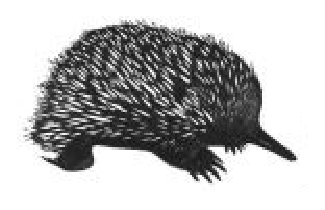
\includegraphics[width=5cm]{pictures/echidna.eps}
\vskip 2cm
{\huge Echidna Documentation}
\end{center}

\tableofcontents
\chapter{Introduction}
\label{ch:intro}

This is the full documentation of the Echidna project, the offline data processing software of the Borexino experiment.
It is meant to be exaustive.
Testers and plain users of the program may bettere jump to \sec{run}.
Module developers may better read \sec{modules}.

The Echidna is a small ant-eater that lives in Australia but Echidna is also the name of a mythological figure of ancient Greece, half woman and half snake she was the daugther of \ldots

The project started in March 2004 and in about six months a working infrastructure was built.
At the moment of writing, about 30 mdoules are operative covering most of the tasks listed above, many of which are currently being tested.

\section{Physics tasks}
\label{sec:intro_tasks}

The main physics goals of the offline code are:
\ben
\item Predecoding (a.k.a. precalibration). Electronics speficic parameters computed for a given run or profile.
\item Decodification of the raw information.
  \ben
  \item Decode GPS time for absolute time reference.
  \item Laben hit time and charge must be inferred from ADC bins using precalibration and calibration data.
  \item The same is true for outer muon hits from TDC bins.
  \item For FADC the parallel operations are pedestal subtraction and the bulding of a digital sum of channels.
    \een
\item Clustering of hits into physical events and precise evealution of event start time. FADC must select the proper windows and provide redundant information.
\item Vertex position reconstruction of the event.
\item Splitting of overlapped events within a cluster.
\item Reconstruction of the event energy.
\item Computation of PID tags:
  \ben
  \item \albe discrimination.
  \item Muon tagging.
  \item Sphericity of the event and other geometrical parameters.
  \een
\item Muon track reconstructions.
\item Calibration tasks:
  \ben 
  \item Single channel calibration: timing and charge for ID and OD.
  \item Dark rate of PMTs.
  \item Scintillator and water quality evaluation.
  \item Electronics status evaluation.
  \item Calibration system auto-monitor.
    \een
\een
and the list is of course not exaustive, nor it can accounts for new ideas being delivered every month as the work proceed.


\section{Design principles}
\label{sec:intro_design}

The guiding principles of the design are:
\bde
\item[Modulary]. 
  The physics algorythms are organized into indipendent modules with a fixed intarface and run by a general engine. 
  The main engine and large set of ancillary routines constitute the \emph{infrastructure} of the program.

\item[Data protection]. 
  Every module is assigned an area with an event class of which it is responsible and it is not allowed (i.e. compilation fails) to write elsewhere. 
  In this way it is immediately possible to track a bug or a mis-computed parameter to its very source.

\item[Use of ROOT]. 
  The collaboration agreed that the official analysis platform in use in Borexino is ROOT\cite{???} . Echidna therefore produces its output as a standard ROOT file. 

\item[Use of Database.] 
  The program is able to access all sort of required information (mapping, geometry, calibration, fluid handling) from the Borexino database.
  A few tables (e.g. precalibration) are also written by echidna.

\item[Single language: C++]. 
  A robust offline program had to be coded using one programming language only and the most natural choice was C++ as it is the language used by ROOT and by its interpreter.
  Moreover the Postgres database to which the program interfaces provides API for C++ and not for Fortran.

\item[\emph{Object-Oriented} (OO) programming]. 
  This design phylosphy comes pretty natural in C++ and constitutes an advantage in enforcing modularity and data protection. 
  However there are different degrees to which it can be pushed and it was decided that the accessibility of the code to a large group of developers was a higher requirement then a truly orthodox OO programming style. 

\item[Network oriented.] 
  Database and rawdata files are accessed over TCP/IP at run time from the DB sever and the disk storage in Gran Sasso\footnote{
    In the future it is foreseen building a mirror in the Lion (France) in2p3 computing facility.} respectively.
  Local copies are needed only if running of an isolated machine.
\ede


\section{Organization}
\label{sec:intro_cycles}

\simfig{cvs_branches}{0.9}{The time evolution of Echidna working cycles.}

The working group is composed of about twenty collaborators, equally distributed among \emph{developers} and \emph{testers}.

Testers have a fundamental role: they have to understanding the module algorythm (from documentaion, without readinbg the code), 
produce a set of relevant simulated and/or real data and perform a list of tests on the module behaviour, finally filling a written report to be archived. 

Every module is assigned a maintaner (usually the author) and a tester.

The interaction among developers working parallely is handled with CVS\footnote{\emph{Concurrent Version System}, a standard tool for this goal\cite{???}.} 
and the code is stored in the official Borexino CVS repository in Gran Sasso.

Under the guide of a project manager, the work is organized in production cycles lasting about 2 months.
Each cycle includes:
\bde
\item[Meeting]. Every cycle starts with a meeting where the \emph{Request-For-Changes} (RFCs) proposed by any co-worker are discussed, approved and scheduled.
\item[Development]. Then a development period of about 6 weeks follows, during which documentation of the code produced must be also supplied and/or updated.
\item[Branch spawning]. When all scheduled tasks have been accomplished the project manager decides to ``freeze'' the code in a parallel CVS branch.
\item[Tests]. A this point testing and debugging occurs on the parallel branch (about 2 weeks), while the main branch remains avalable for further development.
\item[Merging]. At the following cycle meeting testers report on the past branch and if everything is in order the two branches are merged back into one before the next development period starts. 
\ede

\bfig
\includegraphics[angle=90, width=\textwidth]{ech_scheme.eps}
\capfig{scheme}{Echinda general scheme.}
\efig


\chapter{Infrastructure}
%  \input{framework}
  \section{Event Structure}
\label{sec:event_structure}

This section describes only the event structure used internally by echidna.
For the root event structure see \sec{root_event} and \sec{root_event_for_users}.

In this section two concepts are introduced:
\begin{description}
\item{\emph{detector segment}.}
This refers to different components that reflect the Borexino detector structure: ``trigger'', ``laben'', ``muon'', ``fadc'' (flash adc).
Two more segments, ``mctruth'' (Monte Carlo truth) and ``pid'' (particle ID) are also present that do not correspond to a physical DAQ sub-system.  
\item{\emph{reconstruction stage} and \emph{reconstruction step}.}
These refer to the iter the event is undergoing in the program. 
A step brings the event into its next stage.
Reconstruction steps can be: deocoding, clustering, splitting, reconstruction, pulse shape discrimination, ...
Reconstruction steps can be: raw, decoded, clustered, split, reconstructed, discriminated, ...
A module is normally in charge of performing a reconstruction stage.
Different detector segmentss may have different reconstruction steps/stages.
\end{description}

At the moment of writing the structure is not yet frozen; 
particularly it is under discussion the possibility of adding a pseudo-segment called ``global\_event'' 
to collect high level information not related to a particular detector segment.

\bfig
\includegraphics[angle=270, width=\textwidth]{event_structure.eps}
\capfig{event_structure}{Echidna internal event structure.}
\efig

\subsection{Event Classes}

The event structure is depicted in figure \ref{fig:event_structure}.
The most general class in this context is the \code{bx\_echidna\_event}.
This class hosts the event header information and provides relative getters.
Examples of these are the event number, the run number, the crates enabled at run time, ...

Then this class holds 6 objects, one for each detector segment:
\ben
\item \code{bx\_trigger\_event}
\item \code{bx\_laben\_event}
\item \code{bx\_muon\_event}
\item \code{bx\_fadc\_event}
\item \code{bx\_pid\_event}
\item \code{bx\_mctruth\_event}
\een

Every one of the above class inherits from different classes, each one containing information relative to a different reconstruction stage appropriate to that detector segment.
For example the bx\_laben\_event inherits from:
\begin{itemize}
\item \code{bx\_laben\_raw\_event}
\item \code{bx\_laben\_decoded\_event}
\item \code{bx\_laben\_clustered\_event}
\item \code{bx\_laben\_rec\_event}
\end{itemize}

\subsection{Hit Classes}
 
If appropriate a hit class is defined for each reconstruction stage.
In this case the event class holds a vector of these hits.
For example class \code{bx\_laben\_decoded\_event} holds a \code{std::vector<bx\_laben\_decoded\_hits>}, while the getter:

'\code{const bx\_laben\_decoded\_hit\& bx\_laben\_decoded\_event::get\_hit(int i);}' 

returns the hit \#i.

Since the module performing a given reconstruction step may decide to discard hits according to its own criterion, vector of hits in successive reconstruction stages may be disaligned.
For this reason the index is not a good key to retrieve correlated information. 
Instead every hit class has a pointer to its correlated hit in the previous stage.

In addition decoded hit classes have pointers to a \code{db\_channel} object containing database information on the relative channel.
These pointers are assigned by the decoder module the first one in the main loop, therefore they are not available during precalibration.

\subsection{Clusters, Fragments, Windows}

Starting with clustered stage, laben hits are organized in clusters (up to 3 per event) according to the result of clustering modules.
Hits not belonging to any cluster are discarded in this step. 
Clusters refer to physical events within the Borexino trigger gate that are not piled up, i.e. whose time separation is not below 150ns.
Depending on the performance of the splitting module (in development at the time of writing) clusters may be traduced in fragments at a later stage, where also piled up physical events are separeted.

Fadc data are ``naturally'' (i.e. by the daq) organized in windows. 
Windows contain channel objects in early reconstruction stages. 
Clustering for this detector segment limits windows to the 3 most significant ones, hopefully aligned with laben clusters. 

  \section{Raw Event constructors}

The file reader module invokes in cascade the raw event constructors passing them only a pointer to a memory slab where the event has been read from file.
So possibly a raw event constructor can host intellicence necessary to build the raw event.

Generally the first operation every one of the following constructor does, is casting the pointer it recieves to its own \code{struct event\_disk\_format.h}\footnote{see file \code{bx\_event\_disk\_format.h} for details}, so that data words are available in a more user friendly shape.

All constructors return if the first word of their event segment (size) is zero.


\subsection{Trigger}
Words of \code{trigger\_disk\_format} structure are simply copied to analogous private variables, with one exception.
Just before the GPS data, a long word is present, composed by the TAB sum value (16 bits) and by the so called Trigger Word, which is in turn composed by the trgtype (LSB) and by a bitfield with active BTB inputs (MSB). Due to network/host byte ordering conversion the order of these subwords is reversed and the unpacking in this constructor takes care of it.
We find in order:
\begin{enumerate}
\item trg type (8 bits)
\item BTB inputs (8 bits)
\item TAB sum (16 bits)
\end{enumerate}

The BTB input subword is copied into a bitfield to enhace accessibility.


\subsection{Laben}

Simple copy into specular variables, both for the event and for hit class.


\subsection{Muon}

This constructor performs the job of coupling edges into raw hits, a relatively complicated task.

A loop is done over edges, with a step of 2.
Edges reporting \emph{event number}\footnote{these edges are present only for DAQ reasons} or flagged as \emph{invalid} are silently discarded.

A local TDC chip counter is kept and incremented whenever an edge, flagged as \emph{last}, is found; 
the TDC data do not contain information on the board number, so this is evaluted through this chip counter.

A method named \code{m\_check\_validity()} is in charge of checking if the two edges could belong to the same QTC pulse.
It performs 2 checks:
\begin{enumerate}
\item Slopes of the two edges must be different and edges must belong to the same TDC channel. 
If this is not the case then probably an edge was lost. The first edge is then spurious and is being discarded with a debug level message;
the second edge instead could be a valid first edge for the following hit and will be reprocessed. 
Control is returned to the loop which continues with appropriate counter correction.
\item The time ordering of the two edges must be correct, i.e. the first edge time must be higher then the second one
\footnote{Remember that in common stop mode the TDC yields times which go backward from trigger instant.}.
If this is not the case, both edges are simply discarded with a debug level message. 
Control is returned to the loop which simply continues.
This patological behaviour appears usually when an LED is firing at high intensity, resulting in a high after pulse rate. 
\end{enumerate}
If both checks are passed, a raw hit is constructed and pushed into the vector.

The raw hit constructor simply initializes the two edges and the the computed board number.

A final check on TDC chips complains if the total number doesn't meet expectations (8 chips).


\subsection{Fadc}

This contructor copies event level words into analogous variables, then loops over windows to construct them.
A debug level message is issued if no windows are present.

The raw window constructor copies window level words into analogous variables.
If window size is 0, execution is aborted with critic level message.
The number of channels is deduced from data size and window size and channels are constructed in a loop.

The fadc channel constructor simply copies the samples into a private vector.
%  \input{dbi}
%  \input{detector}
% \input{messenger}
  \section{Parameters handling}
\label{sec:parameters}
The known problem of passing informations between unrelated classes in C++ is resolved
in Echidna using a software bus technology which will be explained in this section.

A software bus is an engine to pass informations between objects, called {\it clients}:
in Echidna the class called {\bf bx\_named} is the interface to this bus; every class 
inheriting from bx\_named acquires the access to the bus with the intelligence to read 
parameters from it.

Considering the bus standard topology a {\it master} needs some kind of addressing algoritm to send
the informations only to the relevant objects: in Echidna the address of the client is 
a string, the {\it object name} (from wich bx\_named).
Every bus client is a bx\_named progeny identified in the program by a 
{\bf name}; several istances or implementations with the same name are undistinguished 
from the bus and thus all them have the same parameter set.\\
The bus itself is implemented by the {\bf parameter\_broker} class, while the bus master
job is done by the {\bf configuration\_manager} class; the objects traveling the bus
are {\bf vdt} istances (see \S\ref{sec:vdt}).

This technology is used in Echidna for parameters handling: a parameter is a configuration 
data not hardcoded in the program sources. Parameters are normally initialized in the main
configuration file {\bf echidna.cfg}, set by the current configuration, overrided by the
user configuration file {\bf user.cfg} and by the command line arguments. Parameters differ
from constants which can not be changed without modifying the sources. On the countrary
parameters should not used between modules to pass calculation data (as opposed to 
configuration data): for example the database interface is designed to pass data from 
the precalibrations to the decoding modules.\\
Parameters are identified by their name and organized in {\bf namespaces}: a name has
to be unique in a namespace but a different parameter with the same name can be contained
by a different namespace. The namespace is associated to the bx\_named objects using the
bx\_named names.

\subsection{bx\_named}
The main property of a bx\_named istance is having a name; while a bx\_named object is
useless, since it deal only with parameters, it is an important ancestor for many classes
which parameters.

A name is required to construct a bx\_named object and every class inheriting from bx\_named
must satisfy this requirement in the constructor; the 
\mbox{\code{const string\& bx\_named::get\_name () const}} method can be used
later to retrieve the object name.

The main property of a bx\_named is the access to parameters using the parameter name; 
three methods are present:
\begin{itemize}
\item \mbox{\code{const vdt\& bx\_named::get\_parameter (const std::string\& name) const throw runtime\_error}}:
get the parameter with name \code{name}; the search is limited in the namespace associated to the current
bx\_named. If the search fails an exception (\code{runtime\_error}) is generated. The method is \code{const} and
the return value can not be modified.
\item \mbox{\code{bool bx\_named::check\_parameter (const std::string\& name) const}} is used to check if
the required parameter is present allowing to avoid exception generation if the parameter is absent.
\item \mbox{\code{void bx\_named::set\_parameter (const std::string\& name, const std::string\& value)}} and\\
\mbox{\code{virtual void bx\_named::set\_parameter (const std::string\& name, const vdt\& value)}} are used to set a 
parameter; if the parameter is not already present a warning is issued. The second method is virtual since the 
childs can redefine it to have cached parameters\footnote{Since the access to the parameter requires two
string searches in the parameter\_broker maps, parameter often accessed could be slow and may be better to cache the 
value locally; one example is the bx\_base\_module (\S\ref{sec:modules}) which caches the \code{enable} parameter. 
Redefining that method is not hard: it is important to call \mbox{\code{bx\_named::set\_parameter ()}} method in the 
redefined version to allow the propagation of the parameters in the software bus. 

There is one trick: problems can arise when there are several istances of the same object (with the same name); 
this way calling \mbox{\code{obj1.set\_parameter ()}} affect the cached parameter, the parameter\_broker version, 
but not the version of a obj2 with the same name of obj1. A solution is the use of static cached values even if it can
not be applied always.}
\end{itemize}
For the access to parameters the parameter\_broker is required and thus the bx\_named constructor will generate
an exception if when it's called the broker is not initialized (see below for details on parameter\_broker initializations).

One last method is present: \mbox{\code{bx\_message\& bx\_named::get\_message (bx\_message::message\_level level)}} which
return a bx\_message reference already initialized with the object name and the verbosity levels specified in the parameters.
\subsection{parameter\_broker}
When the configuration files are read no bx\_named object exists yet, so propagating the parameters to the
peers would be impossile; for this reason a parameter broker is present in Echidna: it's role is to receive
the parameters anytime and to distribute them upon request. The parameters are organized in namespaces and 
the relationship between parameter namespaces and bx\_named is the name; each namespace has a name and 
when a client want to fetch a parameter the search is done only in the namespace with same name than the bx\_named
client. This is even the reason for which 2 clients with the same name share the same parameter set.

The parameter namespaces are implemented using a \code{typedef map<string, vdt> parameter\_namespace} and internally
the parameter\_broker keeps the list of namespaces using a \code{map<string, parameter\_namespace>}; no 
access control rule is present in the broker, the setting call only require to know the address (name) of the client.
To avoid acl but to remain in a safe condition the access to the parameter\_broker is allowed only to
bx\_named objects which internals grant runtime access only to the parameter of the target object (the object from
which the set method is called \code{onj.set()}).\\
The parameter\_broker role would suggest a global object, like a singleton, but to keep it available only to bx\_named
clients the pointer to the broker is a static private member of the bx\_named class; this way, once initialized, it will 
be available only to the the bx\_named internals. The initialization is done, by the configuration\_manager, in the 
\mbox{\code{bx\_options::initialize\_echidna ()}} method.

\subsection{configuration\_manager}
Up to here no code is present to read the configuration files, parse them and send the output to the parameter\_broker;
this is the target of the configuration\_manager.

The configuration source in Echidna comes from 2 files and from command line; the explanation of the meaning of these
sources as their format is left to \S\ref{sec:conffile}, here only some important informations are reported:
\begin{enumerate}
\item {\bf echidna.cfg} is the main configuration file organized as a sequence of {\bf stanzas}; each stanza contains 
only the assignement of parameters for bx\_named and can be one of the following type:
\begin{itemize}
\item \code{named}: initialize the contained parameters for the bx\_named with the same name as the stanza
\item \code{module}: as before but the bx\_named is added to the module list
\item \code{config}: a user selectable configuration, containing values to be set for the contained parameters: parameters
are {\bf fully qualified} (their name contain the bx\_named name with the syntax \code{bx\_named\_name.parameter\_name}). 
When a configuration is selected the setting are applied after the initialization of the named/module stanzas. 
The configurations override the default setting for bx\_named parameters.
\end{itemize}
\item {\bf user.cfg} is the user configuration file; it contains only fully qualified parameter assignements.
\item {\bf command line} generates fully qualified parameter assignements with the highest priority.
\end{enumerate}

The configuration\_manger is created in the \mbox{\code{bx\_options::initialize\_echidna ()}} method, which send to it 
the configuration file names and the command line parameters; then the configuration\_manager is ready to upload the 
the parameter\_broker with the parameter with the following order:
\begin{enumerate}
\item initialization stanzas (named and module)
\item configuration stanza for the current configuration (specified on command line)
\item user configuration parameters
\item command line parameters.
\end{enumerate}
The list of module names is also available to be sent to the bx\_module\_factory for the creation of 
the modules, but before this the parameter\_broker pointer has to be stored in the bx\_named static pointer else
no bx\_named object could be created (and thus modules)\footnote{An interesting hack is that the configuration\_manager
inherits from the parameter\_broker; this way the configuration\_manager gets persistent as well as the broker and
even if it is not requested it helps in debugging.}.

  \section{Configuration files and options}
\label{sec:conffile}
The configuration source in Echidna comes from 2 files and from command line, which are processed by the 
configuration\_manager (see \S\ref{sec:parameters}); this section will explain the syntax and the general 
usage of the files and options. 

Parameters leave in namespaces then to identify them is required the namespace name; the choosed syntax is
{\bf namespace\_name.parameter\_name} which is called {\bf Full Qualified Parameter Name} (FQPN).
Since the namespace name is the same as the bx\_named name owning that namespace this syntax
defines the \code{object\_name.parameter\_name} adressing of the parameter.\\
Relative parameter names can be used only inside the bx\_named objects or in the relative initialization
stanzas (see below), elsewhere a parameter is identified by its FQPN.

\subsection{echidna.cfg}
\label{sec:conf_ech_cfg}
It's the main configuration file; it contains the initialization of the program and should never modified 
by users. It contains a list of {\bf stanzas}; empty lines are skipped as well comments starting with the 
character "{\bf \#}".
A stanza is a set of {\bf assegnation lines} preceded and ended by special keywords as in the following examples:
\vskip 2mm
\begin{minipage}{5cm}
\begin{verbatim}
<module bx_laben_decoder>
priority 20
enable 1
discard_out_of_gate_hits 0
disable_lg { }
<end>
\end{verbatim}
\end{minipage}
\begin{minipage}{\textwidth}
start stanza of type {\it module} and name {\it bx\_laben\_decoder}\\
initialize the parameter {\it priority} to {\it 20}\\
initialize the parameter {\it enable} to {\it 1}\\
initialize the parameter {\it discard\_out\_of\_gate\_hits} to {\it 0}\\
initialize the parameter {\it disable\_lg} to an empty vector\\
end the stanza
\end{minipage}
\vskip 2mm

\noindent The first keyword has the form \code{<{\bf stanza\_type} {\bf stanza\_name}>}; stanza\_name is the name 
of the stanza (an arbitrary string from the point of view of the syntax), while stanza\_type is one of \code{named},
\code{module} and \code{config}. Each stanza is ended by the special keyword \code{<end>}.\\
The stanza body is a list of assegnation with the syntax \code{{\bf parameter\_name} {\bf parameter\_value}(s)} 
(one for line) as shown in the previus example; these assegnations assign parameter\_value values to 
the parameter\_name parameters.

The stanza types are:
\begin{itemize}
\item \code{named}: this stanza initializes a parameters namespace whose name is stanza\_name; the role of 
such stanzas is to initialize the default status (parameter values) of bx\_named objects in Echidna.
Each assignement line initialize the specified parameter to the specified value; initializing a parameter
differs from a setting it as explained below and in \sec{custom_param}.

The meaning of the parameters and the accepted types/values fully depend on the target bx\_named objects;
one of the role of these initialization stanzas is to collect the information on the parameters in one file
with their default values (and maybe some comments).

In these stanzas, since the name of the targets bx\_named is well known, the parameter addressing is done only
by the relative parameter name (simply its name).
\item \code{module}: initialize a bx\_base\_module object with name stanza\_name in the same way a named
stanza initialize a bx\_named object. Moreover the specified module is added to the list of objects created by the
module\_factory (\S\ref{sec:modfactory}).
The initialization rules and the paramer addressing rules are the same than in a named stanza.

Some predefined parameters are relevant:
\begin{itemize}
\item \code{enable}: can be 0 or 1 for disabling or enabling the module.
\item \code{priority}: select the priority (integer values) of the module in the framework. The modules with low priority
are executed before modules with high priority.
\end{itemize}
\item \code{config}: create a configuration with name stanza\_name which can be choosed at runtime by Echidna arguments.
Configurations are collection of parameter redefinements whose role is to override the default state of bx\_named 
(and modules) in atomic operations, instead of overriding each parameter manually\footnote{Config stanzas are usefull to
set Echidna in some often used configurations.}

A config stanza body is a list of assegnations where parameter are identified by their FQPN; once a specific configuration
is selected those assignement will be set (not initializated); later reconfiguration can be done by user file or by 
command line.

At list one configuration has to be present, the {\bf default} one (even with empty body); when no other configurations
are specified on command line, this configuration is used.
\end{itemize}

\subsection{user.cfg}
\label{sec:conf_user_cfg}
The role of this file is to specify a set of overrides local to the user. The file consists of
a list of assegnation lines (almost with the same syntax of the config stanza body); parameters
are addressed by their FQPN, empty lines and comments (starting with '\#' character) are skipped.

A small example from my code follows; I normally run without muons, my default file is Run 1612 (with
the specified path) and sometime I happen to disable the \code{bx\_precalib\_laben\_check\_tdc} so that line
is commented.
\begin{verbatim}
bx_event_reader.file_url file:///mnt/scratch/Borex/rawdata/Run001612_01.out.gz
bx_precalib_muon_findpulse.enable 0
bx_precalib_muon_pedestals.enable 0
#bx_precalib_laben_check_tdc.enable 0
bx_muon_decoder.enable 0
\end{verbatim}


\subsection{Echidna inline options}
\label{conf_options}

The main work on options is still to be done, only few options are present actually:
\begin{itemize}
\item \code{-v} increments the Echidna verbosity of one level (\S\ref{sec:messages}); several -v can be
present to increment further the verbosity (actually since the default verbosity value is warn, only
3 -v are usefull).
\item \code{-q} decrement the Echidna verbosity of one level (\S\ref{sec:messages}); several -q can be
present to decrement further the verbosity (actually since the default verbosity value is warn, only
2 -q are usefull). This option is antagonist to -v.
\item \code{-l <file\_path>} specify a logfile with path {\code file\_path}; if file\_path is absent no
logfile is generated.
\item \code{-c file\_path} specifies the path of the user.cfg file (default ./user.cfg)
\item \code{-C file\_path} specifies the path of the echidna.cfg file (default ./echidna.cfg)
\item \code{-p FQPN value} set to value the specified parameter; this assignement has the highest
priority.
\item \code{-f file\_url} set the input file url for the reader, equivalent to "\code{-p bx\_event\_reader.file\_url file\_url}.
\item \code{-o file\_url} set the output file path for the writer, equivalent to "\code{-p bx\_event\_writer.file\_name file\_path}
\item \code{-e max\_number\_of\_events} set the maximum number of processed events.
\end{itemize}

After the options (specified with a '-' character) the first words is the configuration name to be used; this configuration
is checked to be present on the echidna.cfg file and if not an error is issued. Else the specified configuration is
applied; if no configuration is given than the default one is used.
Other fields after the configuration name are meaningless and generate an error.

\subsection{Setting parameter}
\label{sec:conf_param}
The order in with the assignement are applied is relevant and is:
\begin{enumerate}
\item initialization stanzas (named and module)
\item configuration (only the config stanza selected by user)
\item user.cfg
\item command line options specified with -p (or equivalent shortcuts).
\end{enumerate}

The assegnations other than which present in named and module stanzas do not initialize
the parameters; this is not a critical problem. By the way a warning is generated to alert
the user who is setting a uninitializated parameter\footnote{The following warning is issued:\\
\code{\scriptsize
>>> warn: bx\_event\_reader: assigning value to unknown parameter "junk" will initialize it. Check for syntax error
}\\
Which report for an uninitializated parameter \code{junk} and module \code{bx\_event\_reader}.}.

  \section{Root Event}
\label{sec:root_event}

This section describes the \emph{implementation} of the ROOT event in echidna.
Users of the Echidna ROOT file who look for the structure and meaning of variables should intead see \sec{root_event_for_users}. 

\subsection{The Structure}
\label{sec:root_struct}

The event that is being written to the ROOT file is made with a different, though similar, class system 
with respect to the one used internally by Echidna (see \ref{sec:event_structure}).
This class system is depicted in fig.\ref{fig:root_event}.

All classes inherit from \code{TObject} ROOT class and are being provided a dictionary through rootcint utility.
The \code{bx\_writer\_module} (see \ref{sec:writer}) copies each internal event into the same BxEvent class.
The most notable difference here is that, since the event is written in a single step,
the different subobjects do not need to inherit from classes referring to different reconstruction levels.

The structure is straightforward. The main class \code{BxEvent} holds a subobject for every detector segment:
\begin{enumerate}
\item \code{BxTrigger} Info related to the trigger record
\item \code{BxLaben} Info from ID electronics
\item \code{BxMuon} Info from OD electronics
\item \code{BxFadc} Info from FADC electronics (disabled).
\item \code{BxNeutron} Info from Neutron detection system.
\item \code{BxMcTruth} Info from MonteCarlo simulation chain (empty for real data).
\item \code{BxTrackFitted} Muon tracking info fitted from both ID and OD data (empty for non-muons).
\item a vector of \code{BxPhysTags} objects. Written in DSTs by the bxfilter package. $\#0$ for the event $\#1,2\ldots$ for individual clusters.
\end{enumerate}

Some sub-objects, hold the lists of hits and/or clusters\footnote{or fragments or windows.} directly.
Containers for these lists are \code{std::vector<>}.
Nesting vectors putting hits lists inside culster objects currently prevents the benefit of ROOT splitting and is therefore not implemented.
For reconstruction stages where both hits and clusters are present an index variable in the hit class allows the user to know the corresponding cluster. 
Filling containers is fully custumizable by the user with \code{bx\_writer} parameters (see \ref{sec:writer}).

Every event class has:
\begin{enumerate}
\item A default constructor.

This is required by ROOT file I/O. 

\item A working constructor.

This is the only one called explicitly in Echidna. 
It recieves a global flag structure (\code{bx\_write\_opts}) with data lists which are enabled by the user 
and saves into private variables only the flags concerning itself.

\item An assigment operator.

It recieves a refernce to the correspondent internal event object and makes the copy.
\end{enumerate}

The working constructor and the assigment operator are filtered out through conditional compilation when rootcint runs 
and also when the shared object for ROOT is created.
This eliminates the dependency of ROOT event from internal event in this library, essential for using these classes safely within ROOT.

Hit classes do not need assigment operators since the working constructors do everything in this case.

\subsection{ROOT splitting and design choices}
\label{sec:root_split}

This note reports the result of studies on ROOT 
class, tree and file handling and the reasons for choices in the design.
It must be understood only in order to modify the internals, 
while users should skip it completely.

ROOT splitting is a big advantage in terms of file I/O efficiency and of graphical tool functionality (e.g. the \code{TBrowser}), 
so the ROOT classes have been designed keeping it as requirement.

\code{BxEvent} class must hold sub classes as objects,
because pointers are not splitted in the \code{TBranch}
and references are not supported by ROOT at all.
This is connected to the fact that ROOT splitting cannot be done for (possibly) polymorphic objects.
The idea of having a polymorphic light/heavy \code{BxEvent} class has therefore been abandoned.
 
A \code{TClonesArray} in the main event class could be included both as an obj and as ptr,
and it would be split correctly in both cases.
However when placed in sub-obj, a \code{TClonesArray} will be splitted only if included as a pointer. 

In turn using pointers to \code{TClonesArray} requires:
\begin{enumerate}
\item The default constructor must construct the \code{TClonesArray} 
or the \code{TTree::Branch()} will segfault (!!!, internally uses the def ctor to see obj size?)
To avoid memory leaks the size is set to 0 in this context.

\item Calling new/delete for \code{BxEvent} class around the \code{TTree::Fill()} in the writer doesn't work.
This is because ROOT caches the pointer to the \code{TClonesArray} at the \code{TBranch::SetAddress()}, 
and these result invalid if \code{BxEvent} is recreated every time. 
It could be solved with a new \code{TBranch::SetAddress()} at every loop, but it is unacceptably slow.
\end{enumerate}

This last point is the reason why a single event is created in the writer and is being rewritten every time with the assigment operators.

Starting with some version of ROOT later then v4.00 the support for STL conbtainers have been improved.
Therefore TClonesArray have been abandoned for std::vector whose use is more straightforward.
They have to be included as objects in order to be split.
In particular the need for point 1 above is removed.
An attempt to create and destroy the object at every event using vectors has not yet been done and is postponed.

After a large correspondance with P.Canal and R.Brun of the ROOT team, 
it has been assessed that nesting lists of whichever kind prevents splitting of the innermost level 
and the ROOT team is not planning to change this due to the cumbersome maintainance it would require.
This is the reason of having hits outside the cluster objects.

%\input{base_module}

\chapter{Special modules}
  \section{bx\_reader}
\label{sec:reader}

To be done...
  \section{bx\_writer}
\label{sec:writer}

This is a special module regarded as part of the infrastructure of Echidna.

This module handles the ROOT file, the ROOT tree and the ROOT event.

It has the special \code{role=writer}.
It is executed in the main loop after all other modules, i.e. it has the highest priority number.

\subsection{ROOT file} 

A \code{TFile} object is opened in the \code{begin()} method and closed in the \code{end()} method.
The file name is tunable through a user parameter.
The default is "auto", which means that file name will be composed with the std syntax featuring the run number.
If a file with the name requested already exists, by default the program exits with a critic level message, 
unless the proper user parameter to overwrite files is set to true.

Outside the tree, the ROOT file holds also ROOT objects handled by the \code{bx\_root\_barn} (see \ref{sec:barn}).
These are written in the \code{end()} method via \code{bx\_root\_barn::write()} method.


\subsection{ROOT tree}

A \code{TTree} object is created in the \code{begin()} method and written to file in the \code{end()} method.
The ROOT \code{TTree} class is used, since there is no need to develop a dedicated class so far.

A Single \code{TBranch} is created with the \code{BxEvent} class.
Its splitting level\footnote{set to maximum by default.} and buffer size are tunable through user parameters.

The \code{TTree} object is named ``bxtree'', while the \code{TBranch} object is named ``events''.


\subsection{ROOT event}

A single \code{BxEvent} is created in Echidna execution and echidna internal events (\code{bx\_reco\_event}) are copied onto this event before tree is filled.
A technical explanation of this design can be found in \ref{sec:root_event}.

The copy is performed in the \code{doit()} method just before \code{TTree::Fill()} is called. 
It is achieved through the assigment operators defined for \code{BxEvent} class and all its subclasses. 

A helper method \code{m\_parse\_options()} is in charge of reading all user parameters related to which data containers should enabled. 
A struct is filled with these flags and passed to the event constructor.

  %\input{omon}

\chapter{Modules}
  \section{Precalibration: Muon}
\label{sec:precalib_muon}

The outer detector requires two precalibration modules.
They must run in order, in two successive precalibration cycles.

\subsection{bx\_precalib\_muon\_findpulse}

This module simply finds the time\footnote{All times used in precalibration are raw times, i.e. they are unsigned long values expressed in TDC ticks (1.0416ns).} 
of the precalibration pulse in the TDC time window. 
The information in used by the \code{bx\_precalib\_muon\_pedestals} module.

It uses a single private \code{std::vector<unsigned long>} as a time histogram for all channels together.
In the \code{doit()} method the vector is filled with lead times of ordinary channels.
In the \code{end()} method custom algorythms from algorythms.hh are used to make compuations.
Mean value is written to appropriate \code{db\_run} variable.

\code{b\_has\_data} is used to prevent unnecessary computation.

\subsection{bx\_precalib\_muon\_pedestals}

This module computes QTC pedestals for every outer muon channel.
The information is used for charge computation by \code{bx\_muon\_decoder}

It uses a private \code{std::vector<unsigned long>} as a histogram for each channel.
In the \code{doit()} method the vectors are filled with relative times differenses (lead-trail).

3 filters are applied in the following order:
\begin{enumerate}
\item Channel type. Only ordinary channels are processed.
\item Pulse time. Only pulses falling within a tolerance from the preclibration time are accepted.
Precalib pulse time comes from previous precalibration and is retrieved through \code{db\_run} object.
Tolerance is set through user parameter \code{precalib\_pulse\_tolerance}.
\item Pulse width. Only pulse falling between min and max values are accepted. 
A Warning is generated for pulses falling outside.
Min and max values are set through user parameters (\code{min\_pedestal\_width} and \code{max\_pedestal\_width} respectively).
\end{enumerate}

In the \code{end()} method custom algorythms from algorythms.hh are used to make computations.
Mean value is written to appropriate \code{db\_run} variable for every ordinary channel.

\code{b\_has\_data} is used to prevent unnecessary computation.

  \section{bx\_muon\_decoder}

This module performs the decoding of muon data. It requires the muon part of the event to be in the raw stage.
It is friend of the \code{bx\_muon\_decoded\_event} and \code{bx\_muon\_decoded\_hit} class.
At the end of the work the muon event is marked into \code{decoded} stage.

Currently neutrino trgtypes and laser394 trgtypes are handled by two indipendent helper methods:
\begin{enumerate}
\item \code{m\_process\_physics\_event()}
\item \code{m\_process\_laser\_event()}
\end{enumerate}
All other trigger types are discarded with a warning level message.

Possibly the laser event processing will be moved to a dedicated calibration module.

\subsection{physics}

Time is evaluated to TDC gate opening (1 << 13 ticks before trigger), in nanoseconds\footnote{through constant \code{constants::muon::tdc::ns\_per\_clock}}.
Correction for PMT time offset is not yet applied since calibration are not yet completed.
Hits outside the gate (improbable) are discarded.

Charge is evaluated as the TDC time difference (lead-trail), pedestal subtracted, and currently converted in pe with constants measured for 1 QTC channel.
As soon as calibrations will be completed, this will be changed accordingly.

\subsection{laser}

A first quick loop on hits finds the reference channel.
If this is not found the method return with an error level message. 

Time is evaluated as time from LED reference pulse, in nanoseconds\footnote{through constant \code{constants::muon::tdc::ns\_per\_clock}}.
Hits coming before reference pulse are discarded (as well as improbable out of gate hits).

Charge is evaluated as the TDC time difference (lead-trail), pedestal subtracted, and currently converted in pe with constants measured for 1 QTC channel.
The charge calibration strategy is still to be defined

  \section{bx\_baricentrator}
\label{sec:bx_baricentrator}

This module calculates the center of light (baricenter) for each cluster; the baricenter
position is useful for a first estimation of the event vertex from where to start the real
space reconstruction minimization. Only neutrino triggers are handled; clustering is required.

Several algorithms are defined:
\begin{eqnarray}
\vec{B}_Q & = & \frac{N_Q}{n_{hits}} \sum_{i = hits} \tilde{q}_i \vec{x}_i\\
\vec{B}_T & = & \frac{N_T}{n_{hits}} \sum_{i = hits} \frac {\vec{x}_i}{t_i + T_T}\\
\vec{B}_{QT} & = & \frac{N_{QT}}{n_{hits}} \sum_{i = hits} \frac {\tilde{q}_i \vec{x}_i}{t_i + T_{QT}}
\end{eqnarray}
Where $\vec{B}$ is the baricenter position, $\vec{x}_i$ is the position of the photomultiplier which
fired that hit, $\tilde{q}_i$ is the rounded charge of the hit, $t_i$ is the time of the hit (referred to the start
of the cluster) and $n_{hits}$ is the number of hits. The values $N_x$ and $T_x$ are normalization constants for the algorithm, defined as 
module parameters (see echidna.cfg).

The calculation of the center of light is done using the hits in a configurable time gate, 
which should cut off hits from reflections and other delayed processes.
In figure~\ref{fig:cluster_time_distrib} the time distribution of the hits in the clusters is shown;
this pictures comes from a source air run (run 1610). The first reflection peak is at 50ns; to select only
the primary hits the gate should start at 0 and end at about 35ns. The {\bf first\_hits\_gate}
module parameter defines the end of the gate.

\begin{figure}[h]
\begin{center}
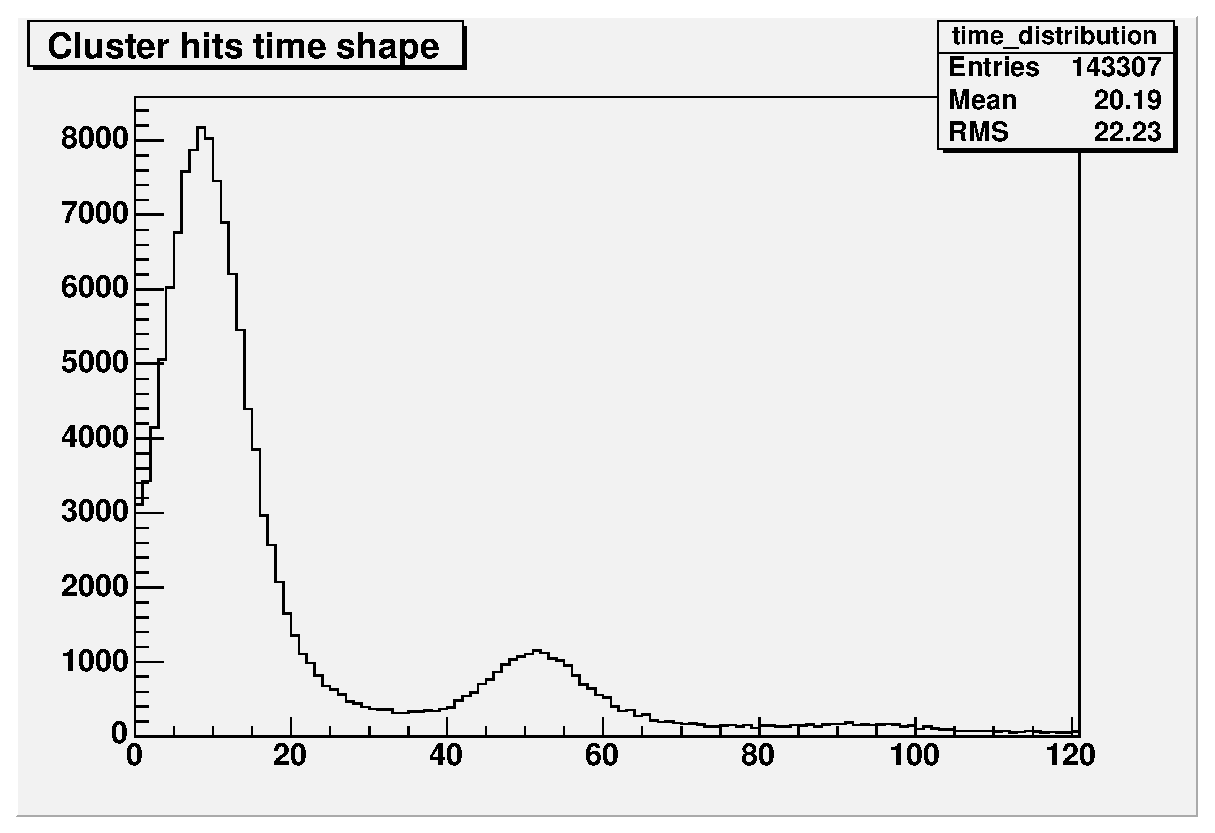
\includegraphics[width=0.8\textwidth]{pictures/cluster_time_distrib}
\caption{Cluster hits time distribution (time in ns)}
\label{fig:cluster_time_distrib}
\end{center}
\end{figure}

The $\tilde{q}_i$ is rounded to integer values starting from $q_i$ as follow: 
\[\tilde{q}_i = \left\{ \begin{array}{ll} 
0 & if\ q_i < q_0 \\
1 & if\ q_i < 0.5\ and\ q_0 < 0.5 \\
round(q_i) & else \\
\end{array}\right.\] 
where $q_0$ is defined by the module parameter {\bf zero\_charge\_limit}. The value of $n_{hits}$ is calculted
according to the algorithm and the charge ($n_{hits} = \sum_{hits} 1$ for T and $n_{hits} = \sum_{i=hits} \tilde{q}_i$ else).

\vskip 2mm
Some other values are defined as follow:
\begin{eqnarray}
\overline{t} & = & \frac{1}{n_{hits}}\sum_{i = hits}\tilde{q}_i\; t_i \\
\overline{tof} & = & \frac{1}{c\; n_{hits}} \sum_{i = hits} \tilde{q}_i\; |\vec{x}_i - \vec{B}| \\
R(t) & = & \sqrt{\frac{1}{n_{hits}}\sum_{i=hits} \tilde{q}_i \; \left[|\vec{x}_i - \vec{B}| - c(t_i + t)\right]^2} \\
t_0 & = & \overline{tof} - \overline{t}
\end{eqnarray}
Where $\tilde{q}_i$ is 1 if T algorithm is used.

$R(t)$ represents an error radius for an event with vertex in the baricenter position at time $t$;
the minimization of $R(t)$ can be done algebraically which leads to $t_{R_{min}} = t_0$. The value of
$t_0$ is a good candidate for the start time of the event and can be calculated very simply as show above.

The real vertex should be searched in the spherical volume with radius $k R_{min}$ and center in the baricenter position, 
where $k$ has to be found sperimentally.


\vskip 2mm
This module outputs the baricenter position (X, Y, Z), $R_{min}$ and $t_0$ in the laben cluster; the histograms
for $R_{min}$ is generated too.







\chapter{User's Guide}
  \section{HOWTO run Echidna}
\label{sec:run}

System requirements: Operating System, CPU, memory, compilers, libraries and packets installed, etc. are defined in Release Notes for every cycle. 

If you are running on the Borexino cluster in Gran Sasso (e.g. on \code{bxmaster}) these requirements are automatically met as the system administrator takes care of it.
However, as mentioned in the cluster tutorial (http://bxweb.lngs.infn.it/echidna/cluster\_tutorial.html), 
this requires that the \code{.bash\_rc} and \code{.bash\_profile} configuration files in your home area are including (sourcing) the file \code{/home/environmental\_setup}.


\subsection{Getting the code}
\label{sec:run_get}

The Echidna code is stored in Borexino official cvs repository in Gran Sasso.

In the Borexino cluster cvs is already set up for you.
Otherwise you simply need to set the following environmental variable:
\qcode{CVSROOT = bxmaster.lngs.infn.it:/home/cvs/}

Then you download the code with the following standard cvs command:
\qcode{cvs co -r cycle\_2 Echidna}
where ``\code{cycle\_2}'' is the name of the branch you want to get.
If you don't specify it (i.e. you omit the \code{-r} option), you get the latest branch.
This may eventually be an unstable developing version, not the right one for testing.


\subsection{Compilation}
\label{sec:run_make}

A Makefile is provided, simply do:
\qcode{make}

This generates three files:
\bde
\item[\code{echidna}]. The executable you will run.
\item[\code{libechinda.so}]. Echidna internal library. 
  Nothing special about it, just leave it in peace.
\item[\code{root/rootechidna.so}]. Echidna ROOT library. 
  You will need to load this into ROOT (after echidna exedcution) when you want to look at the ROOT file echidna has produced for you (\sec{root_event_for_users}). 
\ede


\subsection{Setting up the Database connection}
\label{sec:run_db}

If you are working on Borexino Cluster there is nothing you have to do, skip to next section.

If not, you will need to setup the IP address of the DB server, before you can run.

This can be done adding the following line to the file \code{user.cfg} (\sec{custom_user_cfg}) in the main Echidna directory:
\qcode{bx\_dbi.SERVER1 bxdb.lngs.infn.it}

In addition, the IP address \emph{from}  which you connect to DB must be in the list of authorized addresses of the Postrgres server in Gran Sasso.
If you are working on a machine of an institute of the Borexino collaboration this may be already the case.
If not or if you are running at home, you need to send an email to the cluster administrator with the IP address you want to be authorized.

If you want to use a different DB server (mirrors in other institutions) use that address and contact its system administrator for authorization.

If finally you want to install a local copy of the database, you find instructions in\cite{???}.
Then you will need:
\qcode{bx\_dbi.SERVER1 127.0.0.1}
in your \code{user.cfg} file


\subsection{Running Echidna}
\label{sec:run_run}

You can run echidna calling directly the executable (no launching script is used.):
\qcode{./echidna -f run://XXXX}
where XXXX is the number (not the filename!) of the run you want to process .

The rawdata file will be automatically retrieved through TCP/IP from the official Borexino storage in Gran Sasso.

If you need instead to process a local rawdata file, you can do it with:
\qcode{./echidna -f filename}


  \section{Customizing the execution}
\label{sec:custom}

The user has two possibilities to custumize the behaviour of echidna: a user configuration file and command line options.

Most of this customization involves over-writing the default values of the parameters of a module (or of other infrastructure objects).

The deafult values  are specified in the file named \code{echidna.cfg} (\sec{conf_ech_cfg}), however editing this complex file is discouraged.
One of the two methods described below should be chosen instead.


\subsection{User configuration file}
\label{sec:custom_user_cfg}

A file named \code{user.cfg} is present in the main Echidna directory.
It is inially empty (apart from a comment).
The user is free to edit it and add lines.

Line must have the following syntax:
\qcode{module\_name.parameter\_name parameter\_value}

Empty lines and comments (starting with '\#' character) are skipped.

A small example from my code follows; I normally run without muons, my default file is Run 1612 
and sometime I happen to disable the \code{bx\_precalib\_laben\_check\_tdc} so that line is commented.
\begin{verbatim}
bx_event_reader.file_url run://1612
bx_precalib_muon_findpulse.enable 0
bx_precalib_muon_pedestals.enable 0
#bx_precalib_laben_check_tdc.enable 0
bx_muon_decoder.enable 0
\end{verbatim}


\subsection{Echidna inline options}
\label{sec:custom_options}

Command line options have higher priority with respect to \code{user.cfg} directives. 

The options currently present are:
\begin{itemize}
\item \code{-v} increments the Echidna verbosity of one level (\S\ref{sec:messages}); several -v can be
present to increment further the verbosity (actually since the default verbosity value is warn, only
3 -v are usefull).
\item \code{-q} decrement the Echidna verbosity of one level (\S\ref{sec:messages}); several -q can be
present to decrement further the verbosity (actually since the default verbosity value is warn, only
2 -q are usefull). This option is antagonist to -v.
\item \code{-l <file\_path>} specify a logfile with path {\code file\_path}; if file\_path is absent no
logfile is generated.
\item \code{-c file\_path} specifies the path of the user.cfg file (default ./user.cfg)
\item \code{-C file\_path} specifies the path of the echidna.cfg file (default ./echidna.cfg)
\item \code{-p FQPN value} set to value the specified parameter; this assignement has the highest
priority.
\item \code{-f file\_url} set the input file url for the reader, equivalent to "\code{-p bx\_event\_reader.file\_url file\_url}.
\item \code{-o file\_url} set the output file path for the writer, equivalent to "\code{-p bx\_event\_writer.file\_name file\_path}
\item \code{-e max\_number\_of\_events} set the maximum number of processed events.
\end{itemize}

In addition (and after) the options, the command line accepts also an argument, the ``configuration'' to be used (a string).
These are pre-established sets of parameters defined in \code{echidna.cfg} (\sec{conf_ech_cfg}).
If the argument is not provided, the default configuration is used.

\subsection{Setting parameters}
\label{sec:custom_param}

To summarize, the order in with the parameter values are assigned is relevant:
\begin{enumerate}
\item echidna.cfg (default configuration)
\item configuration (if provided on command line)
\item user.cfg
\item command line options
\end{enumerate}

Trying to assign a value to a non existing parameter (with any method) will issue a warning: 
\qcode{>>> warn: bx\_module\_name: assigning value to unknown parameter "param'' will initialize it. Check for syntax error.}
to alert the user against a probable mispelled directive. 
However note that it is not a critical condition and the execution proceeds.


  \section{Root Event}
\label{sec:root_event_for_users}

This section describes the structure of the ROOT event in detail and from the user point of view.
The type, name and meaning of all variables is reported here.
For details of the implementation and reasons for design choices see \sec{root_event}.

\subsection{Getting started}

After opening ROOT you need to load the echidna ROOT library, before you attempt to open the ROOT file.
Assuming you work in the \code{Echidna} directory, there are three ways to load the library:
\ben
\item Manually in CINT\footnote{The ROOT interactive C++ interpreter, what you get after starting ROOT in a standard way.}:
\qcode{root[0] .L root/rootechidna.so}

\item In your Macro, adding at the beginning:
\qcode{gROOT->LoadMacro("root/libechidna.so");}

\item In your \code{rootlogon.C} file with the same syntax:
\qcode{gROOT->LoadMacro("root/libechidna.so");}
This file (if existing in the current directory) is processed by ROOT at startup.
  If you create this file remember that it must begin and end with a couple of curly braces like an non-named macro.
\een

\simfig{xterm}{0.8}{Basic sequence to browse the Echidna ROOT file}

\subsection{The File structure}

Echidna generated ROOT files include two separate sections: a TTree object and a folder with test histograms.

The latest includes a subfolder for every module that registers at list 1 histogram to the ROOT barn\footnote{
Only if \code{bx\_root\_barn::test} is used at registration instead of \code{bx\_root\_barn::junk} (see \sec{modules})}. 
Every subfolder simply hosts the histograms registered by the module.

The rest of this section deals therefore with the tree object.

This class system is depicted in \fig{root_event}. 

\bfig 
\includegraphics[angle=270, width=0.6\textwidth]{root_event.eps}
\capfig{root_event}{Echidna ROOT event structure.}
\efig
  
The structure is straightforward. The main class \code{BxEvent} holds 8 sub-object:
\ben
\item \code{BxTrigger} Info related to the trigger record
\item \code{BxLaben} Info from ID electronics
\item \code{BxMuon} Info from OD electronics
\item \code{BxFadc} Info from FADC electronics (disabled).
\item \code{BxNeutron} Info from Neutron detection system.
\item \code{BxMcTruth} Info from MonteCarlo simulation chain (empty for real data).
\item \code{BxTrackFitted} Muon tracking info fitted from both ID and OD data (empty for non-muons).
\item a vector of \code{BxPhysTags} objects. Written in DSTs by the bxfilter package. $\#0$ for the event $\#1,2\ldots$ for individual clusters.
\een

Some sub-objects hold the lists of hits and/or clusters\footnote{or fragments or windows.} directly.
Containers for these lists are \code{std::vector<>}.
Nesting vectors (i.e. putting hits lists inside cluster objects) is not done (see technical section \sec{root_event}).
For reconstruction stages where both hits and clusters are present, an index variable in the hit class allows the user to know the corresponding cluster. 
Filling containers is fully custumizable by the user through \code{bx\_writer} module parameters (see \sec{writer}).

The list of physical variables in every class will be described next.

\doublefigs{browser_histo}{0.49}{browser_tree}{0.49}{browser}{The ROOT file as seen by the TBrowser GUI. The histogram (left) and the tree (right) folders are expanded in the two panels.}

\subsection{BxEvent}

private members:\\
\begin{tabular}{ll@{\hspace{2ex}\code{//} }p{8cm}}
\code{    Int\_t        }&\code{run;}&\code{run number}\\
\code{    Int\_t        }&\code{evnum;}&\code{event number (trigger ID)}\\
\code{    UShort\_t     }&\code{enabled\_crates;}&\code{bitfield: 0=trigger, 1-14=laben, 14=muon, 15=fadc;}\\
\code{    BxTrigger     }&\code{trigger;}\\
\code{    BxLaben       }&\code{laben;}\\
\code{    BxMuon        }&\code{muon;}\\
\code{    BxFadc        }&\code{fadc;}\\
\code{    BxMcTruth     }&\code{mctruth;}\\
\code{    BxNeutron     }&\code{neutron;}\\
\code{    BxFittedTrack }&\code{track;}\\
\code{    std::vector<BxPhysTags> }&\code{tags;}&\code{[0] referred to event; [1]...[n] to individual clusters;}\\ 
\end{tabular}

\noindent public getters:\\ 
\begin{tabular}{lll}
\code{    Int\_t             }&\code{GetRun           }&\code{() const;}\\
\code{    Int\_t             }&\code{GetEvNum         }&\code{() const;}\\
\code{    Bool\_t            }&\code{IsCrateEnabled   }&\code{( int i ) const;}\\ 
\code{    UShort\_t          }&\code{GetEnabledCrates }&\code{() const;}\\
\code{    Bool\_t            }&\code{IsMuonEnabled    }&\code{() const;}\\ 
\code{    Bool\_t            }&\code{IsMuonAligned    }&\code{() const;}\\ 
\code{    Bool\_t            }&\code{IsFadcEnabled    }&\code{() const;}\\ 
\code{    Bool\_t            }&\code{IsMcTruthEnabled }&\code{() const;}\\ 
\code{    Bool\_t            }&\code{IsNeutronEnabled }&\code{() const;}\\ 
\code{    const BxTrigger\&  }&\code{GetTrigger  }&\code{() const;}\\
\code{    const BxLaben\&    }&\code{GetLaben    }&\code{() const;}\\
\code{    const BxFadc\&     }&\code{GetFadc     }&\code{() const;}\\
\code{    const BxMuon\&     }&\code{GetMuon     }&\code{() const;}\\
\code{    const BxNeutron\&  }&\code{GetNeutron  }&\code{() const;}\\
\code{    const BxMcTruth\&  }&\code{GetMcTruth  }&\code{() const;}\\
\code{    const BxTrackFitted\&}&\code{GetTrack    }&\code{() const;}\\
\code{    const BxPhysTags\& }&\code{GetPhysTags }&\code{( int i ) const;}\\
\etr
\\
\btr{lll}
\code{    Double\_t          }&\code{GetTimeDifference }&\code{(const BxEvent* prev) const;}\\ 
\code{    Double\_t          }&\code{GetTimeDifference }&\code{(const BxEvent\& prev) const;}\\ 
\code{    Double\_t          }&\code{GetTimeDifference }&\code{(const Ulong\_t* prev\_gps\_times,}\\
&&\code{Double\_t prev\_laben\_trigger\_time) const;}\\ 
\code{    Double\_t          }&\code{GetTimeDifference }&\code{(int current\_cluster,}\\
&&\code{const BxEvent* prev, int prev\_cluster ) const;}\\ 
\code{    Double\_t          }&\code{GetTimeDifference }&\code{(int current\_cluster,}\\
&&\code{const BxEvent\& prev, int prev\_cluster ) const;}\\ 
\code{    Double\_t          }&\code{GetTimeDifference }&\code{(int current\_cluster, const Ulong\_t* prev\_gps\_times,}\\
&&\code{Double\_t prev\_laben\_cluster\_time) const;}\\ 
\end{tabular}

\noindent The first 3 \code{GetTimeDifference(\ldots)} methods work between events, the last 3 between clusters.

\subsection{BxTrigger}

private members:\\
\begin{tabular}{ll@{\hspace{2ex}\code{//} }p{11cm}}
\code{    UChar\_t }&\code{trgtype;       }&\code{trigger type}\\
\code{    UShort\_t}&\code{btb\_threshold;}&\code{BTB threshold, n. of channels}\\
\code{    UChar\_t }&\code{btb\_inputs;   }&\code{BTB active inputs during event. bitfield. 0,1,7 unused; 2=mtb; 3=tct; 4=l355; 5=l266; 6=l394+calib+random;}\\
\code{    ULong\_t }&\code{gps\_times[2]; }&\code{GPS time since 2000.01.01 0:0:0. [0]=seconds, [1]=nanoseconds}\\
\code{    ULong\_t}&\code{trgtime;}&\code{ppc0 cpu time }\\
\end{tabular}

\noindent public getters (trg type and flag):\\
\begin{tabular}{lll}
\code{    UChar\_t         }&\code{ GetTrgType      }&\code{ () const              ; }\\
\code{    Bool\_t          }&\code{ IsTrgType       }&\code{ ( TrgType t ) const   ; }\\
\code{    UChar\_t         }&\code{ GetBtbInputs    }&\code{ () const              ; }\\
\code{    Bool\_t          }&\code{ HasBtbFlag      }&\code{ ( BtbFlag flag ) const; }\\
\end{tabular}

\noindent
The event is flagged with a trigger type according to the trigger generation request which has the highest priority, 
other trigger generation requests, if any, are recorded by the Borexino Trigger Board and saved in \code{btb\_inputs}. 

\noindent
\code{enum TrgType \{}

\btr{lll}
\code{	neutrino}&\code{ = 1,}&\code{ // Std trg of the ID (comparator of the BTB)}\\
\code{	mtb}&\code{ = 2,}&\code{ // Muon Trigger Board (digital OD trigger)}\\
\code{	l355}&\code{ = 4,}&\code{  // Laser 355nm, radial or oblique}\\
\code{	l394}&\code{ = 8}&\code{  // Laser 394nm, timing, radial or oblique}\\
\code{	l266}&\code{ = 16}&\code{  // Laser 266nm, radial or oblique}\\
\code{	calib}&\code{ = 32}&\code{  // Calibration, pulse to Front-End}\\
\code{	random}&\code{ = 64}&\code{  // "Empty" triggers}\\
\code{	neutron}&\code{ = 128}&\code{  //  neutron}\\
\etr

\code{\};}

\noindent
\code{enum BtbFlag \{}

\btr{lll}
\code{  flag\_mtb}&\code{ = 4}&\code{ // Muon Trigger Board (digital OD trigger)}\\
\code{	flag\_neutron}&\code{ = 8}&\code{ // neutron}\\ 
\code{	flag\_l355}&\code{ = 16}&\code{ // Laser 355nm, radial or oblique}\\
\code{	flag\_l266}&\code{ = 32}&\code{ // Laser 266nm, radial or oblique}\\
\code{	flag\_lcr}&\code{ = 64}&\code{ // Laser for timing OR Calibration OR Random}\\
\etr

\code{\};}

\pagebreak[4]

\noindent other public getters:\\*
\btr{lll@{\hspace{2ex}\code{//} }p{7cm}}
\code{  UShort\_t      }&\code{GetBtbThreshold}&\code{() const;}&\code{BTB threshold, n. of channels}\\
\code{  const ULong\_t*}&\code{GetGpsTimes    }&\code{() const;}&\code{Borexino GPS time (UTC) since 2000.01.01}\\
\code{  ULong\_t       }&\code{GetGpsTimeSec  }&\code{() const;}&\code{seconds}\\
\code{  ULong\_t       }&\code{GetGpsTimeNs   }&\code{() const;}&\code{nanoseconds}\\
\code{  time\_t        }&\code{GetTimeT       }&\code{() const;}&\code{seconds since 1970.01.01 according to the time\_t convention,}\\
\code{  Double\_t      }&\code{GetMjd         }&\code{() const;}&\code{Modified Julian Date fractional days since 1858.11.17}\\
\code{  Long\_t        }&\code{GetRunDay      }&\code{() const;}&\code{integer days since the beginning of daq (2007.05.16).}\\
\code{  Float\_t       }&\code{GetSunAltitude }&\multicolumn{2}{l}{\code{(Float\_t\& azimuth) const;}}\\   
&&&\code{returns the sun's zenith angle. the azimuth is written in the argument.}\\
\code{  time\_t        }&\code{GetSunRise     }&\code{() const;}&\code{sunrise of day of the event in time\_t.}\\
\code{  time\_t        }&\code{GetSunSet      }&\code{() const;}&\code{sunset of day of the event in time\_t. }\\
\code{  time\_t        }&\code{GetMidday      }&\code{() const;}&\code{midday of day of the event in time\_t.}\\
\code{  Bool\_t        }&\code{IsDay          }&\code{() const;}&\code{obvious}\\
\code{  Bool\_t        }&\code{IsNight        }&\code{() const;}&\code{obvious}\\
\code{  ULong\_t       }&\code{GetTrgTime     }&\code{() const;}&\code{return ppc0 cpu time }\\
\code{  Bool\_t        }&\code{IsNight        }&\code{() const;}&\code{obvious}\\
\etr


\subsection{BxLaben}

private members:\\
\begin{tabular}{ll@{\hspace{2ex}\code{//} }p{9cm}}
\code{    Int\_t }&\code{empty\_boards;  }&\code{number of empty laben boards, relevant for muons and neutrons; range 0->280;}\\
\code{    Double\_t }&\code{trigger\_time;  }&\code{trigger time from (averaged) reference laben channels;
    Units: ns; range: 0->6.4ms; 0=last gray crossing if < 3.2ms, 0=forelast gray crossing if > 3.2ms}\\
\code{    Double\_t }&\code{laser\_time;    }&\code{laser time from (averaged) reference laben channels;
    Units: ns; range: 0->6.4ms; 0=last gray crossing if < 3.2ms, 0=forelast gray crossing if > 3.2ms}\\
%\code{    Float\_t  }&\code{npe;            }&\code{Sum of all decoded hits charge. 1pe/hit minimum charge assigned.}\\
\code{    Float\_t  }&\code{charge;         }&\code{Sum of all decoded hits charge in photoelectrons}\\
\code{    Int\_t    }&\code{n\_live\_pmts;  }&\code{Number of ordinary channels alive, computed run time;}\\
\code{    Int\_t    }&\code{n\_live\_charge;}&\code{Number of ordinary with good charge signal, computed run time;}\\
\code{    Int\_t    }&\code{n\_hits\_on\_empty;}&\code{Number of hits on empty/dead channels;}\\
\code{    Int\_t    }&\code{n\_raw\_hits;   }&\code{Number of raw hits;(even if vector is not written)}\\
\code{    Int\_t    }&\code{n\_raw\_hits\_flags[7];   }&\code{n\_good, n\_fifo\_full, n\_fifo\_empty, n\_trg\_jump, n\_trg\_jump\_large, n\_trg\_in\_busy, n\_invalid (as from bx\_laben\_raw\_hit::flags)
}\\
\code{    Int\_t    }&\code{n\_invalid\_pmts;  }&\code{number of ordinary channels (and not disabled timing) for which FE or FF is set}\\
\code{    Int\_t    }&\code{n\_invalid\_charge;  }&\code{number of ordinary channels (and not disabled charge) for which FE or FF is set}\\
\code{    Int\_t    }&\code{n\_decoded\_hits;   }&\code{Number of decoded hits;(even if vector is not written)}\\
\code{    Int\_t    }&\code{n\_clusters;   }&\code{Number of clusters, valid for rec clusters as well;(even if vector is not written)}\\
\code{    Int\_t    }&\code{n\_clusters\_muons;   }&\code{number of clusters for neutron algorythm in muon gate (even if vector is not written)}\\
\code{    Int\_t    }&\code{n\_clusters\_found;}&\code{Number of clusters found by algorythm (may differ from previous for high multiplicity events)}\\
\code{    Int\_t    }&\code{n\_clustered\_hits;   }&\code{Number of clustered hits, valid for rec hits as well (even if vector is not written)}\\
%\code{    Float\_t  }&\code{cluster\_window\_limit;}&\code{the maximum window for clustering
%}\\
\code{    Bool\_t   }&\code{has\_raw;       }&\code{= true if raw hits are written in file}\\
\code{    Bool\_t   }&\code{has\_decoded;   }&\code{= true if decoded hits are written in file}\\
\code{    Int\_t    }&\code{has\_clustered; }&\code{= 1 if clusters are written in file; = 2 if also clustered hits are written}\\
\code{    Int\_t    }&\code{has\_rec; }&\code{= 1 if clusters are written in file; = 2 if also clustered hits are written}\\
\code{    Bool\_t   }&\code{is\_tracked;       }&\code{Is the track valid}\\
\end{tabular}
\\
\begin{tabular}{lll}
\code{    std::vector<BxLabenRawHit>          }&\code{raw\_hits;}\\
\code{    std::vector<BxLabenDecodedHit>      }&\code{decoded\_hits;}\\
\code{    std::vector<BxLabenCluster>         }&\code{clusters;}\\
\code{    std::vector<BxLabenCluster>         }&\code{clusters\_muons;}\\
\code{    std::vector<BxLabenClusteredHit>    }&\code{clustered\_hits;}\\
\code{    std::vector<BxLabenRecCluster>      }&\code{rec\_clusters;}\\
\code{    std::vector<BxLabenRecClusteredHit> }&\code{rec\_hits;}\\
\code{	  BxTrackByPoints                     }&\code{track;}\\
\end{tabular}

\noindent public getters:\\
\begin{tabular}{lll}
\code{    Int\_t    }&\code{GetEmptyBoards }&\code{() const; }\\
\code{    Double\_t }&\code{GetTriggerTime }&\code{() const; }\\
\code{    Double\_t }&\code{GetLaserTime   }&\code{() const; }\\
\code{    Int\_t    }&\code{GetNLivePmts   }&\code{() const; }\\
\code{    Int\_t    }&\code{GetNLiveCharge }&\code{() const; }\\
\code{    Int\_t    }&\code{NormalizePmts  }&\code{(Int\_t arg) const; }\\
\code{    Float\_t  }&\code{NormalizePmts  }&\code{(Float\_t arg) const; }\\
\code{    Float\_t  }&\code{NormalizeCharge}&\code{(Float\_t arg) const; }\\
%\code{    Float\_t  }&\code{GetNpe         }&\code{() const; }\\
\code{    Float\_t  }&\code{GetCharge      }&\code{() const; }\\
%\code{    Float\_t  }&\code{GetClusterWindowLimit}&\code{() const; }\\
\code{    Int\_t    }&\code{GetNHitsOnEmpty}&\code{() const; }\\
\code{    Int\_t    }&\code{GetNRawHits    }&\code{() const; }\\
\code{    Int\_t    }&\code{GetNGood       }&\code{() const; }\\
\code{    Int\_t    }&\code{GetNFifoFull   }&\code{() const; }\\
\code{    Int\_t    }&\code{GetNFifoEmpty  }&\code{() const; }\\
\code{    Int\_t    }&\code{GetNTrgJump    }&\code{() const; }\\
\code{    Int\_t    }&\code{GetNTrgJumpLarge }&\code{() const; }\\
\code{    Int\_t    }&\code{GetNTrgInBusy  }&\code{() const; }\\
\code{    Int\_t    }&\code{GetNInvalid    }&\code{() const; }\\
\code{    Int\_t    }&\code{GetNInvalidPmts}&\code{() const; }\\
\code{    Int\_t    }&\code{GetNInvalidCharge }&\code{() const; }\\
\code{    Int\_t    }&\code{GetNDecodedHits}&\code{() const; }\\
\code{    Int\_t    }&\code{GetNClusters   }&\code{() const; }\\
\code{    Int\_t    }&\code{GetNClustersMuons}&\code{() const; }\\
\code{    Int\_t    }&\code{GetNClustersFound}&\code{() const; }\\
\code{    Int\_t    }&\code{GetNClusteredHits}&\code{() const; }\\
\code{    Bool\_t   }&\code{IsTracked        }&\code{() const; }\\
\code{    Bool\_t   }&\code{HasRawHits       }&\code{() const; }\\
\code{    Bool\_t   }&\code{HasDecodedHits   }&\code{() const; }\\
\code{    Bool\_t   }&\code{HasClusters      }&\code{() const; }\\
\code{    Bool\_t   }&\code{HasClusteredHits }&\code{() const; }\\
\code{    Bool\_t   }&\code{HasRecClusters   }&\code{() const; }\\
\code{    Bool\_t   }&\code{HasRecHits       }&\code{() const; }\\
\end{tabular}\\
\begin{tabular}{lll}
\code{    const std::vector<BxLabenRawHit>\&       }&\code{GetRawHits   }&\code{() const; }\\
\code{    const std::vector<BxLabenDecodedHit>\&   }&\code{GetDecodedHits}&\code{() const; }\\
\code{    const std::vector<BxLabenCluster>\&      }&\code{GetClusters   }&\code{() const; }\\
\code{    const std::vector<BxLabenCluster>\&      }&\code{GetClustersMuons }&\code{() const; }\\
\code{    const std::vector<BxLabenClusteredHit>\& }&\code{GetClusteredHits}&\code{() const; }\\
\code{    const std::vector<BxLabenRecCluster>\&   }&\code{GetRecClusters }&\code{() const; }\\
\code{    const std::vector<BxLabenRecHit>\&       }&\code{GetRecHits }&\code{() const; }\\

\code{    BxLabenRawHit\&       }&\code{GetRawHit       }&\code{(Int\_t i) const; }\\
\code{    BxLabenDecodedHit\&   }&\code{GetDecodedHit   }&\code{(Int\_t i) const; }\\
\code{    BxLabenCluster\&      }&\code{GetCluster      }&\code{(Int\_t i) const; }\\
\code{    BxLabenCluster\&      }&\code{GetClusterMuon         }&\code{(Int\_t i) const; }\\
\code{    BxLabenClusteredHit\& }&\code{GetClusteredHit }&\code{(Int\_t i) const; }\\
\code{    BxLabenRecCluster\&   }&\code{GetRecCluster   }&\code{(Int\_t i) const; }\\
\code{    BxLabenRecHit\&       }&\code{GetRecHit       }&\code{(Int\_t i) const; }\\
\code{    BxTrackByPoints\&     }&\code{GetTrack        }&\code{() const; }\\
\end{tabular}

\subsubsection{BxLabenRawHit}

private members:\\
\begin{tabular}{ll@{\hspace{2ex}\code{//} }p{11cm}}
\code{    UShort\_t }&\code{lg;    }&\code{logical channel (1 based)}\\
\code{    UChar\_t  }&\code{time1; }&\code{First triangular waveform sampling (ADC bins, 0-255)}\\
\code{    UChar\_t  }&\code{time2; }&\code{Second (~80ns later) triangular waveform sampling (ADC bins, 0-255)}\\
\code{    UShort\_t }&\code{gray;  }&\code{Gray counter read out in bins 0->(1<<16-1)}\\
\code{    UChar\_t  }&\code{base;  }&\code{Baseline charge sampling (ADC bins 0-255)}\\
\code{    UChar\_t  }&\code{peak;  }&\code{Peak (~80ns later) charge sampling (ADC bins 0-255)}\\
\code{    UChar\_t  }&\code{order; }&\code{Order in channel as in daq fifo; 1-based}\\
\code{    UChar\_t  }&\code{flags\_board; }&\code{Flags of board header: 1 = N.TRG not consecutive, 2 = N.TRG > DELTA, 3 = TRG in BUSY, 4 = DPR FULL, 5 = FIFO EMPTY, 6 = FIFO FULL}\\
\code{    UChar\_t  }&\code{flags\_ch; }&\code{5 = FIFO EMPTY, 6 = FIFO FULL, 7 = INVALID }\\
\code{    UShort\_t }&\code{errors;    }&\code{Bitfield. Laben error codes}\\
\end{tabular}

\newpage
\noindent public getters:\\
\begin{tabular}{lll@{\hspace{2ex}\code{//} }l}
\code{    UShort\_t }&\code{GetLg    }&\code{() const; }\\
\code{    UChar\_t  }&\code{GetTime1 }&\code{() const; }\\
\code{    UChar\_t  }&\code{GetTime2 }&\code{() const; }\\
\code{    UShort\_t }&\code{GetGray  }&\code{() const; }\\
\code{    UChar\_t  }&\code{GetBase  }&\code{() const; }\\
\code{    UChar\_t  }&\code{GetPeak  }&\code{() const; }\\
\code{    UChar\_t  }&\code{GetOrder }&\code{() const; }\\
\code{    UShort\_t }&\code{GetErrors}&\code{() const; }\\
\code{    UChar\_t  }&\code{GetFlagsBoard  }&\code{() const; }\\
\code{    UChar\_t  }&\code{GetFlagsChannel}&\code{() const; }\\
\code{    Bool\_t   }&\code{IsGood         }&\code{() const; }&\code{flags\_board and flags\_ch with no bits set}\\
\code{    Bool\_t   }&\code{HasFifoFull    }&\code{() const; }&\code{flags\_ch bit 6}\\
\code{    Bool\_t   }&\code{HasFifoEmpty   }&\code{() const; }&\code{flags\_ch bit 5}\\
\code{    Bool\_t   }&\code{HasTrgJump     }&\code{() const; }&\code{flags\_board bit 1}\\
\code{    Bool\_t   }&\code{HasTrgJumpLarge}&\code{() const; }&\code{flags\_board bit 2}\\
\code{    Bool\_t   }&\code{HasTrgInBusy   }&\code{() const; }&\code{flags\_board bit 3}\\
\code{    Bool\_t   }&\code{IsInvalid      }&\code{() const; }&\code{flags\_board bit 7}\\
\end{tabular}

\subsubsection{BxLabenDecodedHit}

private members:\\
\begin{tabular}{ll@{\hspace{2ex}\code{//} }p{11cm}}
\code{    UShort\_t }&\code{lg;          }&\code{logical channel (1 based) }\\
\code{    UShort\_t }&\code{run;         }&\code{run number }\\
\code{    Double\_t }&\code{raw\_time;   }&\code{hit time; Units: ns; range: 0->6.4ms; 0=last gray crossing if < 3.2ms, 0=forelast gray crossing if > 3.2ms}\\
%\code{    Float\_t  }&\code{time\_error; }&\code{0-0.5 hit time validity (good if <0.4)}\\
\code{    UChar\_t  }&\code{flag;        }&\code{Flag for out\_of\_gate=1, reflection=2, reference=4, retrigger=8, disabled=16;}\\
%\code{    Float\_t  }&\code{d80;         }&\code{Real 80ns gap in ns (from time2-time1)}\\
\code{    Float\_t  }&\code{raw\_charge; }&\code{peak-base in bins (without pileup corr.)}\\
\code{    Float\_t  }&\code{charge;      }&\code{photoelectrons (with pileup corr.)}\\
\code{    Float\_t  }&\code{charge\_mean;}&\code{photoelectrons normalized with mean (with pileup corr.)}\\
\code{    Int\_t    }&\code{npe;         }&\code{number of photoelectrons (with a threshold)}\\
\code{    UChar\_t  }&\code{order;       }&\code{Order in channel counting decoded hits only; 1-based}\\
\code{    UShort\_t }&\code{raw\_index;  }&\code{Index in vector of corresponding raw hit}\\
\code{    UShort\_t }&\code{num\_cluster;}&\code{Number of cluster the hit belongs to}\\
\code{    Float\_t  }&\code{rec\_time;   }&\code{Time after TOF subtraction}\\
\code{    Float\_t   }&\code{short\_cluster;}&\code{Flag to say if the hit belonged to the old (c11) clustering}\\
\end{tabular}

\newpage
\noindent public getters:\\
\begin{tabular}{lll}
\code{    UShort\_t }&\code{GetLg        }&\code{() const; }\\
\code{    Double\_t }&\code{GetRawTime   }&\code{() const; }\\
%\code{    Float\_t  }&\code{GetTimeError }&\code{() const; }\\
%\code{    Float\_t  }&\code{GetD80       }&\code{() const; }\\
\code{    UChar\_t  }&\code{GetFlag      }&\code{() const; }\\
\code{    Bool\_t   }&\code{IsGood       }&\code{() const; }\\
\code{    Bool\_t   }&\code{IsOutOfGate  }&\code{() const; }\\
\code{    Bool\_t   }&\code{IsReflection }&\code{() const; }\\
\code{    Bool\_t   }&\code{IsReference  }&\code{() const; }\\
\code{    Bool\_t   }&\code{IsRetrigger  }&\code{() const; }\\
\code{    Float\_t  }&\code{GetRawCharge }&\code{() const; }\\
\code{    Float\_t  }&\code{GetCharge    }&\code{() const; }\\
\code{    Float\_t  }&\code{GetChargeMean}&\code{() const; }\\
\code{    Int\_t    }&\code{GetNpe       }&\code{() const; }\\
\code{    UChar\_t  }&\code{GetOrder     }&\code{() const; }\\
\code{    UShort\_t }&\code{GetRawIndex  }&\code{() const; }\\
\code{    UShort\_t }&\code{GetNumCluster}&\code{() const; }\\
\code{    Float\_t  }&\code{GetRecTime   }&\code{() const; }\\
\code{    Float\_t  }&\code{IsShortCluster}&\code{() const; }\\
\end{tabular}

\subsubsection{BxLabenCluster}

private members:\\
\begin{tabular}{ll@{\hspace{2ex}\code{//} }p{8cm}}
\code{    Int\_t   }&\code{npmts;       }&\code{number of hit pmts}\\
\code{    Int\_t   }&\code{npmts\_conc; }&\code{number of hit pmts with light concentrator }\\
\code{    Int\_t   }&\code{npmts\_thresh;}&\code{number of hit pmts above threshold}\\
\code{    Int\_t   }&\code{npmts\_short;}&\code{number of hit pmts (old c11 clustering)}\\
\code{    Int\_t   }&\code{nhits;       }&\code{number of hits}\\
\code{    Int\_t   }&\code{nhits\_conc; }&\code{number of hits with light concentrators}\\
\code{    Int\_t   }&\code{nhits\_thresh;}&\code{number of hits above threshold}\\
\code{    Int\_t   }&\code{nhits\_short;}&\code{number of hits in old (c11) clustering style}\\
\code{    Int\_t   }&\code{nhits\_bkg;  }&\code{number of dark noise hits estimated to contribute to cluster (mostly relevant for neutrons)}\\
%\code{    Int\_t   }&\code{npe;         }&\code{number of photoelectrons}\\
%\code{    Int\_t   }&\code{npe\_conc;   }&\code{number of photoelectrons with light concentrators}\\
\code{    Float\_t }&\code{charge;      }&\code{photoelectron charge}\\
\code{    Float\_t }&\code{charge\_conc;}&\code{photoelectron charge with light concentrator}\\
\code{    Float\_t }&\code{charge\_mean;}&\code{photoelectron charge normalized to mean}\\
\code{    Float\_t }&\code{charge\_thresh;}&\code{photoelectron charge using only hits above threshold}\\
\code{    Float\_t }&\code{charge\_short;}&\code{photoelectron charge in old (c11) clustering style}\\
\code{    Double\_t }&\code{start\_time; }&\code{cluster start time;
ns; range: $0\rightarrow6.4ms$; 0=last gray crossing if $< 3.2ms$, 0=forelast gray crossing if $> 3.2ms$}\\
%\code{    Double\_t }&\code{rough\_time; }&\code{cluster rough start time ($16ns$ bins); same units as above}\\
\code{    Float\_t }&\code{mean\_time;  }&\code{cluster mean time in ns relative to start\_time}\\
\code{    Float\_t }&\code{mean\_time\_short;}&\code{cluster mean time in ns relative to old (c11) clustering style}\\
\code{    Float\_t }&\code{rms\_time;   }&\code{cluster rms time in ns relative to mean\_time}\\
\code{    Float\_t }&\code{rms\_time\_short;}&\code{cluster rms time in ns relative to mean\_time (old c11 clustering)}\\
\code{    Float\_t }&\code{duration;}&\code{time of the last hit in ns relative to start time}\\
\code{    Float\_t }&\code{duration\_short;}&\code{time of the last hit in ns relative to start time (old c11 clutering)}\\
\code{    UChar\_t   }&\code{flag;      }&\code{Flag for out\_of\_gate=1, broad=2, trigger=4}\\
\code{    UShort\_t  }&\code{decoded\_index; }&\code{Index in vector of decoded hit corresponding to first hit}\\
\end{tabular}

\begin{tabular}{ll@{\hspace{2ex}\code{//} }p{6cm}}

\code{    Int\_t   }&\code{npeaks;       }&\code{number of peaks identified by the splitting algorythm}\\
\code{    Float\_t   }&\code{msk\_nphotons; }&\code{Out-of-fit photons from the msk energy reco (in 4pi)}\\
\code{    BxPosition }&\code{baricenter;    }&\code{reconstructed position from baricentrator}\\
\code{    BxPosition }&\code{position\_mi;  }&\code{reconstructed position from Milano reco}\\
\code{    BxPosition }&\code{position\_lngs;}&\code{reconstructed position from LNGS reco}\\
\code{    BxPosition }&\code{position\_dbn; }&\code{reconstructed position from Dubna reco}\\
\code{    BxPosition }&\code{position\_msk; }&\code{reconstructed position from Moscow reco}\\
\code{    BxPosition }&\code{position\_mach4; }&\code{reconstructed position from Mach4 reco, variable index}\\
\code{    BxPosition }&\code{position\_mach4\_fixed; }&\code{reconstructed position from Mach4 reco, fixed index}\\
\code{    BxEnergy   }&\code{energy\_mc;    }&\code{reconstructed energy from MC reco}\\
\code{    BxEnergy   }&\code{energy\_lik;   }&\code{reconstructed energy from Likelihood reco}\\
\code{    BxEnergy   }&\code{energy\_msk;   }&\code{reconstructed energy from Moscow reco}\\
\code{    BxEnergy   }&\code{energy\_dbn;   }&\code{reconstructed energy from Dubna reco}\\
\code{    std::vector<Float\_t>}&\code{peak\_times;}&\code{times of the peaks found by splitting algorithm in ns form cluster start time.}\\
\code{    std::vector<Float\_t>}&\code{peak\_charges;}&\code{charge of the peaks found by the splitting algorythm in pe.}\\
\end{tabular}

\newpage
\noindent public getters:\\*
\begin{tabular}{lll}
\code{    Int\_t   }&\code{GetNpmts     }&\code{() const; }\\
\code{    Int\_t   }&\code{GetNpmtsConc }&\code{() const; }\\
\code{    Int\_t   }&\code{GetNpmtsThresh }&\code{() const; }\\
\code{    Int\_t   }&\code{GetNpmtsShort }&\code{() const; }\\
\code{    Int\_t   }&\code{GetNHits     }&\code{() const; }\\
\code{    Int\_t   }&\code{GetNHitsConc }&\code{() const; }\\
\code{    Int\_t   }&\code{GetNHitsThresh }&\code{() const; }\\
\code{    Int\_t   }&\code{GetNHitsShort }&\code{() const; }\\
\code{    Int\_t   }&\code{GetNHitsBkg }&\code{() const; }\\
\code{    Int\_t   }&\code{GetNHitsCorr }&\code{() const;    nhits-nhits\_bkg}\\
%\code{    Int\_t   }&\code{GetNpe       }&\code{() const; }\\
%\code{    Int\_t   }&\code{GetNpeConc   }&\code{() const; }\\
\code{    Float\_t }&\code{GetCharge    }&\code{() const; }\\
\code{    Float\_t }&\code{GetChargeConc}&\code{() const; }\\
\code{    Float\_t }&\code{GetChargeThresh}&\code{() const; }\\
\code{    Float\_t }&\code{GetChargeMean}&\code{() const; }\\
\code{    Float\_t }&\code{GetChargeShort}&\code{() const; }\\
\code{    Double\_t}&\code{GetStartTime }&\code{() const; }\\
%\code{    Double\_t}&\code{GetRoughTime }&\code{() const; }\\
\code{    Float\_t }&\code{GetMeanTime  }&\code{() const; }\\
\code{    Float\_t }&\code{GetMeanTimeShort}&\code{() const; }\\
\code{    Float\_t }&\code{GetRMSTime   }&\code{() const; }\\
\code{    Float\_t }&\code{GetRMSTimeShort}&\code{() const; }\\
\code{    Float\_t }&\code{Duration   }&\code{() const; }\\
\code{    Float\_t }&\code{DurationShort}&\code{() const; }\\
\code{    UChar\_t }&\code{GetFlag      }&\code{() const; }\\
\code{    Bool\_t  }&\code{IsGood       }&\code{() const; }\\
\code{    Bool\_t  }&\code{IsOutOfGate  }&\code{() const; }\\
\code{    Bool\_t  }&\code{IsBroad      }&\code{() const; }\\
\code{    Bool\_t  }&\code{IsTrigger    }&\code{() const; }\\
\code{    UShort\_t}&\code{GetDecodedIndex}&\code{() const; }\\
\code{    Int\_t   }&\code{GetNPeaks      }&\code{() const; }\\
\code{    Float\_t }&\code{GetMskNPhotons }&\code{() const; }\\
\code{    const BxPosition\& }&\code{GetBaricenter  }&\code{() const; }\\
\code{    const BxPosition\& }&\code{GetPositionMi  }&\code{() const; }\\
\code{    const BxPosition\& }&\code{GetPositionLNGS}&\code{() const; }\\
\code{    const BxPosition\& }&\code{GetPositionDbn }&\code{() const; }\\
\code{    const BxPosition\& }&\code{GetPositionMsk }&\code{() const; }\\
\code{    const BxPosition\& }&\code{GetPositionMach4 }&\code{() const; }\\
\code{    const BxPosition\& }&\code{GetPositionMach4Fixed }&\code{() const; }\\
\code{    const BxEnergy  \& }&\code{GetEnergyMc    }&\code{() const; }\\
\code{    const BxEnergy  \& }&\code{GetEnergyLik   }&\code{() const; }\\
\code{    const BxEnergy  \& }&\code{GetEnergyMsk   }&\code{() const; }\\
\code{    const BxEnergy  \& }&\code{GetEnergyDbn   }&\code{() const; }\\
\code{    Float\_t }&\code{GetPeakTime   }&\code{( Int\_t i ) const; }\\
\code{    Float\_t }&\code{GetPeakCharge }&\code{( Int\_t i ) const; }\\
\code{    const std::vector<Float\_t>\&  }&\code{GetPeakTimes   }&\code{() const; }\\
\code{    const std::vector<Float\_t>\&  }&\code{GetPeakCharges }&\code{() const; }\\
\end{tabular}

\subsubsection{BxLabenClusteredHit}

private members:\\
\begin{tabular}{ll@{\hspace{2ex}\code{//} }p{10cm}}
\code{    UShort\_t }&\code{lg;          }&\code{logical channel (1 based) }\\
\code{    UShort\_t }&\code{run;         }&\code{run number }\\
\code{    Int\_t }&\code{num\_cluster; }&\code{Cluster (1,2,3) the hit belongs to}\\
\code{    Float\_t }&\code{time;     }&\code{Time relative to cluster start time in ns}\\
\code{    Float\_t }&\code{charge;     }&\code{photoelectrons (with pileup corr.)}\\
\code{    Float\_t }&\code{charge\_mean;     }&\code{photoelectrons normalized with mean (with pileup corr.)}\\
\code{    UChar\_t }&\code{order;          }&\code{Order in channel; Only hits in cluster counted; 1-based}\\
\code{    UShort\_t }&\code{decoded\_index;}&\code{Index in vector of corresponding decoded hit}\\
\end{tabular}

\noindent public getters:\\*
\begin{tabular}{lll}
\code{    UShort\_t }&\code{GetLg          }&\code{() const; }\\
\code{    Int\_t    }&\code{GetNumCluster  }&\code{() const; }\\
\code{    Float\_t  }&\code{GetTime        }&\code{() const; }\\
\code{    Float\_t  }&\code{GetCharge      }&\code{() const; }\\
\code{    Float\_t  }&\code{GetChargeMean  }&\code{() const; }\\
\code{    UChar\_t  }&\code{GetOrder       }&\code{() const; }\\
\code{    UShort\_t }&\code{GetDecodedIndex}&\code{() const; }\\
\end{tabular}

\subsubsection{BxPosition}

private members:\\
\begin{tabular}{ll@{\hspace{2ex}\code{//} }p{10cm}}
\code{    Float\_t }&\code{time;   }&\code{time of event start from fit, no standard zero available yet\footnote{One will be specified soon, meanwhile see specific module documentation.}}\\
\code{    Float\_t }&\code{x;      }&\code{x from fit (m)}\\
\code{    Float\_t }&\code{y;      }&\code{y from fit (m)}\\
\code{    Float\_t }&\code{z;      }&\code{z from fit (m)}\\
\code{    Float\_t }&\code{dt;     }&\code{dt from fit (m)}\\
\code{    Float\_t }&\code{dx;     }&\code{dx from fit (m)}\\
\code{    Float\_t }&\code{dy;     }&\code{dy from fit (m)}\\
\code{    Float\_t }&\code{dz;     }&\code{dz from fit (m)}\\
\code{    Float\_t }&\code{user;   }&\code{mi: likelihood, value of the fcn at the minimum (normalized); mach4: index of refraction}\\
\code{    Bool\_t  }&\code{converged;}&\code{Fit converged}\\
\code{    Int\_t   }&\code{matrix; }&\code{ Matrix def pos (+1), approximate (0) or not def pos (-1)}\\
\end{tabular}

\newpage
\noindent public getters:\\
\begin{tabular}{llll}
    \code{    Float\_t }&\code{GetTime}  & \code{() const; } \\
    \code{    Float\_t }&\code{GetX   }  & \code{() const; } \\
    \code{    Float\_t }&\code{GetY   }  & \code{() const; } \\
    \code{    Float\_t }&\code{GetZ   }  & \code{() const; } \\
    \code{    Float\_t }&\code{GetDT  }  & \code{() const; } \\
    \code{    Float\_t }&\code{GetDX  }  & \code{() const; } \\
    \code{    Float\_t }&\code{GetDY  }  & \code{() const; } \\
    \code{    Float\_t }&\code{GetDZ  }  & \code{() const; } \\
    \code{    Float\_t }&\code{GetDR  }  & \code{() const; }&\code{in-getter conversion} \\ 
    \code{    Float\_t }&\code{GetTheta} & \code{() const; }&\code{in-getter conversion} \\
    \code{    Float\_t }&\code{GetPhi  } & \code{() const; }&\code{in-getter conversion} \\
    \code{    Float\_t }&\code{GetLikelihood } & \code{() const; } \\
    \code{    Float\_t }&\code{GetRefIndex   } & \code{() const; } \\
    \code{    Float\_t }&\code{GetUser       } & \code{() const; } \\
    \code{    Int\_t   }&\code{GetMatrix     } & \code{() const; } \\
    \code{    Bool\_t  }&\code{IsDefPos      } & \code{() const; } \\
    \code{    Bool\_t  }&\code{IsNotDefPos   } & \code{() const; } \\
    \code{    Bool\_t  }&\code{IsApproximate } & \code{() const; } \\
    \code{    Bool\_t  }&\code{IsConverged   } & \code{() const; } \\
    \code{    Float\_t }&\code{GetDistance} & \code{(const BxPosition\& p) const; } \\
    \code{    Float\_t }&\code{GetDistance} & \code{(const BxTrackByPoints\& t) const; } \\
\end{tabular}

\subsubsection{BxEnergy}

private members:\\
\begin{tabular}{ll@{\hspace{2ex}\code{//} }l}
\code{    Int\_t   }&\code{nhits;       }&\code{nhits corrected for position }\\
\code{    Int\_t   }&\code{npe;         }&\code{npe corrected for position }\\
\code{    Float\_t }&\code{charge;      }&\code{charge corrected for position }\\
\end{tabular}

\noindent public getters:\\
\begin{tabular}{llll}
    \code{    Int\_t   }&\code{GetNHits  }& \code{() const; } \\
    \code{    Int\_t   }&\code{GetNpe    }& \code{() const; } \\
    \code{    Float\_t }&\code{GetCharge }& \code{() const; } \\
\end{tabular}

\subsubsection{BxLabenRecCluster}

private members:\\
\begin{tabular}{ll@{\hspace{2ex}\code{//} }p{9cm}}
\code{    Float\_t }&\code{ns\_asymmetry;}&\code{north-south charge asymmetry}\\
\code{    Float\_t }&\code{sphere\_chi2; }&\code{chi2 to sphericity}\\
\code{    Float\_t }&\code{sphere\_lkl;  }&\code{likelihood to sphericity}\\
\code{    Float\_t }&\code{sphere\_rel\_var;}&\code{relative variance = sigma/mean of the hits in the cos(theta) - phi plane centered in the event position and normalized per hit charge. 0 to 2 approx}\\
\code{    Float\_t }&\code{plane\_cos;}&\code{cos of the angle made by the plane fitting the theta-phi parameters space}\\
\code{    Float\_t }&\code{plane\_chi2;}&\code{chi2/NDF of the fit of a plane in a cos(theta)-phi distribution}\\
\code{    Float\_t }&\code{h\_plane\_chi2; }&\code{chi2/NDF of the fit of a horizontal plane in a cos(theta)-phi distribution}\\
\code{    Float\_t }&\code{sh\_power[4];  }&\code{power of spherical armonics}\\
\code{    Char\_t  }&\code{quality\_flags;}&\code{bitfield, meaning to be assigned}\\
\code{    Float\_t }&\code{tailtot[10];  }&\code{tailtot for tail value 40-130ns step 10ns}\\
\code{    Float\_t }&\code{gatti;        }&\code{gatti optimal filter variable}\\
\code{    Float\_t }&\code{gattic;       }&\code{gatti optimal filter variable (cumulative)}\\
\code{    Float\_t }&\code{lkl;          }&\code{likelihood ratio}\\
\code{    Float\_t }&\code{lklc;         }&\code{likelihood ratio (cumulative)}\\
\code{    Float\_t }&\code{rise\_time;   }&\code{rise time}\\
\code{    Float\_t }&\code{tailtot\_mach4[10];}&\code{tailtot for tail value 30-110ns step 5ns}\\
\code{    Float\_t }&\code{gatti\_mach4[4];   }&\code{gatti optimal filter variable from 4 reference shapes}.\\
\code{    Float\_t }&\code{peak\_mach4;       }&\code{peak of tof-recorrected hit time distribution}\\
\code{    Float\_t }&\code{mean\_mach4;       }&\code{mean of tof-recorrected hit time distribution}\\
\code{    Float\_t }&\code{rms\_mach4;        }&\code{rms of tof-recorrected hit time distribution}\\
\code{    Float\_t }&\code{skew\_mach4;       }&\code{skewness of tof-recorrected hit time distribution}\\
\code{    Float\_t }&\code{kurt\_mach4;       }&\code{kurtosis of tof-recorrected hit time distribution}\\
\end{tabular}

\newpage
\noindent public getters:\\

\begin{tabular}{lll}
\code{    Float\_t }&\code{GetNsAsymmetry }&\code{() const; }\\
\code{    Float\_t }&\code{GetSphereChi2  }&\code{() const; }\\
\code{    Float\_t }&\code{GetSphereLkl   }&\code{() const; }\\
\code{    Float\_t }&\code{GetSphereRelVal}&\code{() const; }\\
\code{    Float\_t }&\code{GetPlaneCos    }&\code{() const; }\\
\code{    Float\_t }&\code{GetPlaneChi2   }&\code{() const; }\\
\code{    Float\_t }&\code{GetHPlaneChi2  }&\code{() const; }\\
\code{    Float\_t }&\code{GetSHPower     }&\code{(int order) const; }\\
\code{    Char\_t }&\code{GetQualityFlags }&\code{() const; }\\
\code{    const Float\_t* }&\code{GetTailTot}&\code{() const; }\\
\code{    Float\_t }&\code{GetTailTot     }&\code{(Int\_t tail) const; }\\
\code{    Float\_t }&\code{GetGatti       }&\code{() const; }\\
\code{    Float\_t }&\code{GetGattiC      }&\code{() const; }\\
\code{    Float\_t }&\code{GetLkl         }&\code{() const; }\\
\code{    Float\_t }&\code{GetLklC        }&\code{() const; }\\
\code{    Float\_t }&\code{GetRiseTime       }&\code{() const; }\\
\code{    const Float\_t* }&\code{GetTailTotMach4}&\code{() const; }\\
\code{    Float\_t }&\code{GetTailTotMach4}&\code{(Int\_t tail) const; }\\
\code{    Float\_t }&\code{GetGattiMach4  }&\code{() const; }\\
\code{    Float\_t }&\code{GetMeanMach4   }&\code{() const; }\\
\code{    Float\_t }&\code{GetPeakMach4   }&\code{() const; }\\
\code{    Float\_t }&\code{GetRMSMach4    }&\code{() const; }\\
\code{    Float\_t }&\code{GetSkewMach4   }&\code{() const; }\\
\code{    Float\_t }&\code{GetKurtMach4   }&\code{() const; }\\
\end{tabular}

\subsubsection{BxLabenRecHit}

private members:\\
\begin{tabular}{ll@{\hspace{2ex}\code{//} }p{10cm}}
\code{    UShort\_t }&\code{lg;          }&\code{logical channel (1 based) }\\
\code{    UShort\_t }&\code{run;         }&\code{run number }\\
\code{    Int\_t }&\code{num\_cluster; }&\code{Cluster (1,2,3) the hit belongs to}\\
\code{    Float\_t }&\code{time;     }&\code{Time relative to cluster start time in ns}\\
\code{    UChar\_t }&\code{order;          }&\code{Order in channel; Only hits in cluster counted; 1-based}\\
\code{    UShort\_t }&\code{decoded\_index;}&\code{Index in vector of corresponding decoded hit}\\
\end{tabular}

\noindent public getters:\\
\begin{tabular}{lll}
\code{    UShort\_t }&\code{GetLg          }&\code{() const; }\\
\code{    Int\_t    }&\code{GetNumCluster  }&\code{() const; }\\
\code{    Float\_t  }&\code{GetTime        }&\code{() const; }\\
\code{    UChar\_t  }&\code{GetOrder       }&\code{() const; }\\
\code{    UShort\_t }&\code{GetDecodedIndex}&\code{() const; }\\
\end{tabular}


\subsection{BxMuon}

private members:\\
\begin{tabular}{ll@{\hspace{2ex}\code{//} }p{9cm}}
\code{    Bool\_t  }&\code{is\_aligned;               }&\code{did not loose sycronicyty}\\
\code{    Int\_t   }&\code{n\_raw\_hits;              }&\code{number of raw hits (even if vector is not written)}\\
\code{    Int\_t   }&\code{n\_decoded\_hits;          }&\code{number of decoded hits (even if vector is not written)}\\
\code{    Int\_t   }&\code{n\_clusters;               }&\code{number of clusters (even if vector is not written)}\\
\code{    Int\_t   }&\code{n\_clustered\_hits\_sss;   }&\code{number of clustered hits on sss (even if vector is not written)}\\
\code{    Int\_t   }&\code{n\_clustered\_hits\_floor; }&\code{number of clustered hits on floor (even if vector is not written)}\\
\code{    Int\_t   }&\code{decoded npmts;   }&\code{number of fired pmts after decoding}\\
\code{    Float\_t }&\code{decoded charge;  }&\code{photoelectron charge after decoding}\\
\code{    Bool\_t  }&\code{has\_cluster\_sss;  }&\code{data present}\\
\code{    Bool\_t  }&\code{has\_cluster\_floor;}&\code{data present}\\
\code{    Int\_t   }&\code{npmts;          }&\code{number of fired pmts}\\
\code{    Float\_t }&\code{start\_time\_sss;    }&\code{cluster start time from clustering module; Units: ns; 0=trigger\_time+8500;}\\
\code{    Float\_t }&\code{start\_time\_floor;  }&\code{cluster start time from clustering module; Units: ns; 0=trigger\_time+8500;}\\
\code{    Float\_t }&\code{charge\_sss;    }&\code{photoelectron charge on sss}\\
\code{    Float\_t }&\code{charge\_floor;  }&\code{photoelectron charge on floor}\\
\code{    Bool\_t  }&\code{is\_tracked;    }&\code{track present}\\
\code{    Bool\_t  }&\code{has\_raw;       }&\code{= true if raw hits are written in file}\\
\code{    Bool\_t  }&\code{has\_decoded;   }&\code{= true if decoded hits are written in file}\\
\code{    Bool\_t  }&\code{has\_clustered; }&\code{= 1 if clusters are written; = 2 if clustered hits are written in file}\\
\end{tabular}
\\
\begin{tabular}{lll}
\code{    std::vector<BxMuonRawHit>       }&\code{raw\_hits;}\\
\code{    std::vector<BxMuonDecodedHit>   }&\code{decoded\_hits;}\\
\code{    std::vector<BxMuonCluster>      }&\code{clusters;}\\
\code{    std::vector<BxMuonClusteredHit> }&\code{clustered\_hits;}\\
\code{    BxTrackByPoints                 }&\code{track;}\\
\end{tabular}

\newpage
\noindent public getters:\\
\begin{tabular}{lll}
\code{    Bool\_t }&\code{IsAligned             }&\code{() const; }\\
\code{    Int\_t  }&\code{GetNRawHits           }&\code{() const; }\\
\code{    Int\_t  }&\code{GetNDecodedHits       }&\code{() const; }\\
\code{    Int\_t  }&\code{GetNClusters          }&\code{() const; }\\
\code{    Int\_t  }&\code{GetNClusteredHitsSSS  }&\code{() const; }\\
\code{    Int\_t  }&\code{GetNClusteredHitsFloor}&\code{() const; }\\
\code{    Int\_t  }&\code{GetNClusteredHits     }&\code{() const; }\\
\code{    Int\_t  }&\code{GetDecodedNPmts       }&\code{() const; }\\
\code{    Float\_t}&\code{GetDecodedCharge      }&\code{() const; }\\
\code{    Bool\_t }&\code{HasClusterSSS         }&\code{() const; }\\
\code{    Bool\_t }&\code{HasClusterFloor       }&\code{() const; }\\
\code{    Bool\_t }&\code{HasCluster            }&\code{() const; }\\
\code{    Int\_t  }&\code{GetNPmts              }&\code{() const; }\\
\code{    Float\_t}&\code{GetStartTimeSSS       }&\code{() const; }\\
\code{    Float\_t}&\code{GetStartTimeFloor     }&\code{() const; }\\
\code{    Float\_t}&\code{GetStartTime          }&\code{() const; }\\
\code{    Float\_t}&\code{GetChargeSSS          }&\code{() const; }\\
\code{    Float\_t}&\code{GetChargeFloor        }&\code{() const; }\\
\code{    Float\_t}&\code{GetCharge             }&\code{() const; }\\
\code{    Bool\_t }&\code{IsTracked             }&\code{() const; }\\
\code{    Bool\_t }&\code{HasRaw                }&\code{() const; }\\
\code{    Bool\_t }&\code{HasDecoded            }&\code{() const; }\\
\code{    Bool\_t }&\code{HasClustered          }&\code{() const; }\\
\code{    const std::vector<BxMuonRawHit>\&     }&\code{GetRawHits     }&\code{() const; }\\
\code{    const std::vector<BxMuonDecodedHit>\& }&\code{GetDecodedHits }&\code{() const; }\\
\code{    const std::vector<BxMuonClusteredHit>\&}&\code{GetClusteredHits }&\code{() const; }\\
\code{    const std::vector<BxMuonCluster>\&    }&\code{GetClusters }&\code{() const; }\\
\code{    BxTrackByPoints\&                     }&\code{GetTrack }&\code{() const; }\\
\end{tabular}

\subsubsection{BxMuonRawHit}

private members:\\
\begin{tabular}{ll@{\hspace{2ex}\code{//} }p{11cm}}
\code{    UShort\_t }&\code{mch;        }&\code{muon channel (0-255)}\\
\code{    ULong\_t  }&\code{lead\_time;  }&\code{leading edge time in TDC ticks (1.0416ns); range: 0->8192}\\
\code{    ULong\_t  }&\code{trail\_time; }&\code{trailing edge time in TDC ticks (1.0416ns); range: 0->8192}\\
\end{tabular}

\noindent public getters:\\
\begin{tabular}{lll}
\code{    UShort\_t }&\code{GetMch       }&\code{() const; }\\
\code{    Float\_t  }&\code{GetLeadTime  }&\code{() const; }\\
\code{    Float\_t  }&\code{GetTrailTime }&\code{() const; }\\
\end{tabular}

\subsubsection{BxMuonDecodedHit}

private members:\\
\begin{tabular}{ll@{\hspace{2ex}\code{//} }p{13cm}}
\code{    UShort\_t }&\code{run;    }&\code{run number}\\
\code{    UShort\_t }&\code{mch;    }&\code{muon channel (0-255)}\\
\code{    Float\_t  }&\code{time;   }&\code{time after gate start (neutrino) or led ref (laser); ns; $0\rightarrow8.5\mu s$}\\
\code{    Float\_t  }&\code{charge; }&\code{Charge (pe)}\\
\end{tabular}

\noindent public getters:\\
\begin{tabular}{lll}
\code{    UShort\_t }&\code{GetMch    }&\code{() const; }\\
\code{    Float\_t  }&\code{GetTime   }&\code{() const; }\\
\code{    Float\_t  }&\code{GetCharge }&\code{() const; }\\
\end{tabular}

\subsubsection{BxMuonClusteredHit}

private members:\\
\begin{tabular}{ll@{\hspace{2ex}\code{//} }p{12cm}}
\code{    UShort\_t }&\code{run;    }&\code{run number}\\
\code{    UShort\_t }&\code{mch;    }&\code{muon channel (0-255)}\\
\code{    Float\_t  }&\code{time;   }&\code{time after gate start (neutrino) or after led ref (laser); ns; 0->8.5$\mu s$}\\
\code{    Float\_t  }&\code{charge; }&\code{charge (pe)}\\
\end{tabular}

\noindent public getters:\\
\begin{tabular}{lll}
\code{    UShort\_t }&\code{GetMch    }&\code{() const; }\\
\code{    Float\_t  }&\code{GetTime   }&\code{() const; }\\
\code{    Float\_t  }&\code{GetCharge }&\code{() const; }\\
\end{tabular}

\subsubsection{BxMuonCluster}

private members:\\
\begin{tabular}{ll@{\hspace{2ex}\code{//} }l}
\code{    Int\_t   }&\code{id;          }&\code{internal cluster id}\\
\code{    Float\_t }&\code{x;           }&\code{x of charge baricenter, exp time weighted}\\
\code{    Float\_t }&\code{y;           }&\code{y of charge baricenter, exp time weighted}\\
\code{    Float\_t }&\code{z;           }&\code{z of charge baricenter, exp time weighted}\\
\code{    Float\_t }&\code{start\_time; }&\code{time of first hit, ns after gate start}\\
\code{    Float\_t }&\code{charge;      }&\code{sum of hits charge, pe}\\
\end{tabular}

\pagebreak[4]

\noindent public getters:\\*
\begin{tabular}{lll@{\hspace{2ex}\code{//} }p{10cm}}
\code{    Int\_t   }&\code{GetId        }&\code{() const; }\\
\code{    Float\_t }&\code{GetX         }&\code{() const; }\\
\code{    Float\_t }&\code{GetY         }&\code{() const; }\\
\code{    Float\_t }&\code{GetZ         }&\code{() const; }\\
\code{    Float\_t }&\code{GetRadius    }&\code{() const; }&\code{Baricenter distance from origin}\\
\code{    Float\_t }&\code{GetRc        }&\code{() const; }&\code{Baricenter distance from origin on x-y plane}\\
\code{    Float\_t }&\code{GetPhi       }&\code{() const; }&\code{Baricenter Phi, in-getter computation}\\
\code{    Float\_t }&\code{GetTheta     }&\code{() const; }&\code{Baricenter Theta, in-getter computation}\\
\code{    Float\_t }&\code{GetStartTime }&\code{() const; }\\
\code{    Float\_t }&\code{GetCharge    }&\code{() const; }\\
\code{    Bool\_t  }&\code{IsUp         }&\code{() const; }&\code{Baricenter on upper SSS}\\
\code{    Bool\_t  }&\code{IsDown       }&\code{() const; }&\code{Baricenter on lower SSS}\\
\code{    Bool\_t  }&\code{IsSSS        }&\code{() const; }&\code{Baricenter on SSS}\\
\code{    Bool\_t  }&\code{IsFloor      }&\code{() const; }&\code{Baricenter on Floor}\\
\end{tabular}


\subsection{BxFadc}

private members:\\
\begin{tabular}{ll@{\hspace{2ex}\code{//} }p{10cm}}
\code{    UChar\_t }&\code{event\_flag;        }&\code{DAQ event flag; see table \ref{tab:fadc_flag}  for possible values; }  \\
\code{    Float\_t }&\code{time\_to\_previous; }&\code{time to the previous event in 20 ns units}  \\
\code{    Float\_t }&\code{trigger\_time;      }&\code{fited time from the trigger ramp channel; units fdac ticks (2.5ns); 0 is trigger; }  \\
\code{    Int\_t }&\code{has\_raw;       }&\code{=1 if windows are written in file; =2 if also channels are written }  \\
\code{    Int\_t }&\code{has\_decoded;   }&\code{=1 if windows are written in file; =2 if also channels are written }  \\
\code{    Int\_t }&\code{has\_clustered; }&\code{=1 if windows are written in file; =2 if also channels are written }  \\
\end{tabular}
\\
\begin{tabular}{lll}
\code{    std::vector<BxFadcRawWindow>      }&\code{raw\_windows; }  \\
\code{    std::vector<BxFadcRawChannel>     }&\code{raw\_channels; } \\
\code{    std::vector<BxFadcDecodedWindow>  }&\code{decoded\_windows; }\\
\code{    std::vector<BxFadcDecodedChannel> }&\code{decoded\_channels; }\\
\code{    std::vector<BxFadcDecodedWindow>  }&\code{clustered\_windows; }\\
\code{    std::vector<BxFadcDecodedChannel> }&\code{clustered\_channels; }\\
\end{tabular}

\btab
\begin{tabular}{c|l}
\hline
  value       &      DAQ condition\\
\hline 
 0 & event rejected without even reading total sum;\\
 1 & event rejected because it contains no significant data;\\
 2 & event contained window(s) above noise level;\\
 4 & event is in a coincidence;\\
 6 & event above WIN\_THRESHOLD and in a coincidence with a later one;\\
 7 & event above WIN\_THRESHOLD and in a coincidence with a previous one;\\
 8 & event above EVENT threshold;\\
16 & at least 1 board has erroneous trigger count;\\
32 & at least 1 board has erroneous pattern value;\\
64 & V896 times are inconsistent.\\
\hline 
\end{tabular}
\captab{fadc_flag}{Possible fadc event\_flag values (from DAQ). 6 is the minimum to keep an event;}
\etab

\pagebreak[4]

\noindent public getters:\\*
\begin{tabular}{lll}
\code{    UChar\_t }&\code{GetEventFlag      }&\code{() const; }\\
\code{    Float\_t }&\code{GetTimeToPrevious }&\code{() const; }\\
\code{    Float\_t }&\code{GetTriggerTime    }&\code{() const; }\\
\code{    Bool\_t }&\code{HasRawWindows        }&\code{() const; }\\
\code{    Bool\_t }&\code{HasRawChannels       }&\code{() const; }\\
\code{    Bool\_t }&\code{HasDecodedWindows    }&\code{() const; }\\
\code{    Bool\_t }&\code{HasDecodedChannels   }&\code{() const; }\\
\code{    Bool\_t }&\code{HasClusteredWindows  }&\code{() const; }\\
\code{    Bool\_t }&\code{HasClusteredChannels }&\code{() const; }\\
\code{    const std::vector<BxFadcRawWindow>\&      }&\code{GetRawWindows        }&\code{() const; }\\
\code{    const std::vector<BxFadcRawChannel>\&     }&\code{GetRawChannels       }&\code{() const; }\\
\code{    const std::vector<BxFadcDecodedWindow>\&  }&\code{GetDecodedWindows    }&\code{() const; }\\
\code{    const std::vector<BxFadcDecodedChannel>\& }&\code{GetDecodedChannels   }&\code{() const; }\\
\code{    const std::vector<BxFadcDecodedWindow>\&  }&\code{GetClusteredWindows  }&\code{() const; }\\
\code{    const std::vector<BxFadcDecodedChannel>\& }&\code{GetClusteredChannels }&\code{() const; }\\
\end{tabular}

\subsubsection{BxFadcRawChannel}

private members:\\
\begin{tabular}{ll@{\hspace{2ex}\code{//} }p{11cm}}
\code{   Int\_t }&\code{num\_window;     }&\code{number of window the channel belongs to}\\
\code{   UChar\_t }&\code{samples[4096]; }&\code{raw samples, height of signal every 2.5ns in bins (range 0-255)}\\
\end{tabular}

\noindent public getters:\\
\begin{tabular}{lll}
\code{    Int\_t   }&\code{GetNumWindow     }&\code{() const; }\\
\code{    UChar\_t }&\code{GetSample (Int\_t i) const; }\\
\end{tabular}

\subsubsection{BxFadcRawWindow}

private members:\\
\begin{tabular}{ll@{\hspace{2ex}\code{//} }p{12cm}}
\code{    ULong\_t  }&\code{length; }&\code{data size in bytes}\\
\code{    UChar\_t  }&\code{flag; }&\code{flag for window position in memory page; 0=in page; 1=starting with page; 2=ending with page; 3=1\&\&2;}\\
\code{    Short\_t  }&\code{begin; }&\code{window start time with respect to trigger; negative; in 2.5ns units}\\
\code{    UShort\_t }&\code{size; }&\code{window size; in 2.5ns units}\\
\end{tabular}

\noindent public getters:\\
\begin{tabular}{lll}
\code{    ULong\_t  }&\code{GetLength }&\code{() const; }\\
\code{    UChar\_t  }&\code{GetFlag   }&\code{() const; }\\
\code{    Short\_t  }&\code{GetBegin  }&\code{() const; }\\
\code{    UShort\_t }&\code{GetSize   }&\code{() const; }\\
\end{tabular}

\subsubsection{BxFadcDecodedChannel}

private members:\\
\begin{tabular}{ll@{\hspace{2ex}\code{//} }p{11cm}}
\code{    Int\_t   }&\code{num\_window; }&\code{number of window the channel belongs to}\\
\code{    Float\_t }&\code{amplitude;   }&\code{height at maximum signal amplitude}\\
\code{    Float\_t }&\code{charge;      }&\code{integral of signal; arbitrary units}\\
\code{    Float\_t }&\code{peak;        }&\code{time of peak; 0 is window start; units: fadc ticks (2.5ns).}\\
\end{tabular}

\noindent public getters:\\
\begin{tabular}{lll}
\code{    Int\_t   }&\code{GetNumWindow }&\code{() const; }\\
\code{    Float\_t }&\code{GetAmplitude }&\code{() const; }\\
\code{    Float\_t }&\code{GetPeak      }&\code{() const; }\\
\code{    Float\_t }&\code{GetCharge    }&\code{() const; }\\
\end{tabular}

\subsubsection{BxFadcDecodedWindow}

private members:\\
\begin{tabular}{ll@{\hspace{2ex}\code{//} }p{7cm}}
\code{    UChar\_t  }&\code{flag;   }&\code{flag for window position in memory page; 0=in page; 1=starting with page; 2=ending with page; 3=1\&\&2;}\\
\code{    UChar\_t  }&\code{status; }&\code{result of the second peak search: 1=no other pulse; 2=1 more pulse before main one; 3=1 more pulse after main one; 4=2\&\&3;}\\
\code{    Short\_t  }&\code{begin;  }&\code{start time with respect to trigger; negative; in 2.5ns units}\\
\code{    UShort\_t }&\code{size;   }&\code{window time span; units: fadc ticks (2.5 ns);}\\
\code{    BxFadcDecodedChannel }&\code{sum; }&\code{digital sum virtual channel}\\
\code{    Float\_t }&\code{sum\_samples[4096]; }&\code{digital sum samples, height of signal every 2.5ns in bins (range 0-255)}\\
\end{tabular}

\noindent public getters:\\
\begin{tabular}{lll}
\code{    UChar\_t  }&\code{GetFlag   }&\code{() const; }\\
\code{    UChar\_t  }&\code{GetStatus }&\code{() const; }\\
\code{    Short\_t  }&\code{GetBegin  }&\code{() const; }\\
\code{    UShort\_t }&\code{GetSize   }&\code{() const; }\\
\code{    const }&\code{BxFadcDecodedChannel\& GetSum }&\code{() const; }\\
\code{    Float\_t  }&\code{GetSumSample  }&\code{(Int\_t i); } \\
\end{tabular}

\subsection{BxMcTruth}

private members:\\
\begin{tabular}{ll@{\hspace{2ex}\code{//} }p{12cm}}
\code{    Int\_t }&\code{n\_hits\_id;  }&\code{ number hits in ID (even if vector is not written)}\\
\code{    Int\_t }&\code{n\_hits\_od;  }&\code{ number hits in OD (even if vector is not written)}\\
\code{    Int\_t }&\code{n\_daughters; }&\code{ number daughters (even if vector is not written)}\\
\code{    Int\_t }&\code{n\_deposits;  }&\code{ number deposits (even if vector is not written)}\\
\code{    Int\_t }&\code{n\_users;     }&\code{ number users (even if vector is not written)}\\
\code{    Int\_t }&\code{n\_frames;    }&\code{ number frames (even if vector is not written)}\\
\code{    Int\_t }&\code{write\_flag;  }&\code{=1 if frames are written in file; =2 if also hits, daughters, deposits and users are written}\\
\end{tabular}
\\
\begin{tabular}{lll}
\code{    std::vector<BxMcTruthFrame>   }&\code{frames;   }\\
\code{    std::vector<BxMcTruthDaughter>}&\code{daughters;}\\
\code{    std::vector<BxMcTruthDeposit> }&\code{deposits; }\\
\code{    std::vector<BxMcTruthUser>    }&\code{users;    }\\
\code{    std::vector<BxMcTruthHit>     }&\code{hits\_id; }\\
\code{    std::vector<BxMcTruthHit>     }&\code{hits\_od; }\\
\end{tabular}

\noindent public getters:\\
\begin{tabular}{lll}
\code{    Int\_t  }&\code{GetNHitsId    }&\code{() const; }\\
\code{    Int\_t  }&\code{GetNHitsOd    }&\code{() const; }\\
\code{    Int\_t  }&\code{GetNFrames    }&\code{() const; }\\
\code{    Int\_t  }&\code{GetNDaughters }&\code{() const; }\\
\code{    Int\_t  }&\code{GetNDeposits  }&\code{() const; }\\
\code{    Int\_t  }&\code{GetNUsers     }&\code{() const; }\\
\code{    Bool\_t }&\code{HasFrames     }&\code{() const; }\\
\code{    Bool\_t }&\code{HasHits       }&\code{() const; }\\
\code{    BxMcTruthFrame\& }&\code{GetFrame      }&\code{(Int\_t i) const; }\\
\code{    const std::vector<BxMcTruthFrame>\&    }&\code{GetFrames    }&\code{() const; }\\
\code{    const std::vector<BxMcTruthDaughter>\& }&\code{GetDaughters }&\code{() const; }\\
\code{    const std::vector<BxMcTruthDeposit>\&  }&\code{GetDeposits  }&\code{() const; }\\
\code{    const std::vector<BxMcTruthUser>\&     }&\code{GetUsers     }&\code{() const; }\\
\code{    const std::vector<BxMcTruthHit>\&      }&\code{GetHitsId    }&\code{() const; }\\
\code{    const std::vector<BxMcTruthHit>\&      }&\code{GetHitsOd    }&\code{() const; }\\
\end{tabular}

\subsubsection{BxMcTruthFrame}

Each (eventually piled up) physical particle is associated to a frame
\noindent private members:\\ 
\begin{tabular}{ll@{\hspace{2ex}\code{//} }p{10cm}}
\code{    UShort\_t }&\code{file\_id;         }&\code{progressive number for bx\_elec input files. o-based.}\\
\code{    Double\_t }&\code{elec\_event\_time;}&\code{relative to trg time, ns}\\
\code{    Int\_t    }&\code{event\_id;        }&\code{event number in bx\_elec input file.}\\
\code{    Int\_t    }&\code{n\_sequence;      }&\code{Sequence number of isotope in the chain, 1 based}\\
\code{    Int\_t    }&\code{isotope\_coinc;   }&\code{1 if it's part of a chain, related to his father by dt<??h ($\rightarrow$same position), 0 otherwise.}\\
\code{    Int\_t    }&\code{pdg;              }&\code{Particle Data Group Code of the Particle}\\
\code{    Double\_t }&\code{time;             }&\code{Absolute time after run start, ns}\\
\code{    Float\_t  }&\code{energy;           }&\code{Kinetic energy, MeV}\\
\code{    Float\_t  }&\code{visible\_energy;  }&\code{Quenched energy, MeV}\\
\code{    Float\_t  }&\code{position  [3]     }&\code{3D vector of the particle generation point, m}\\
\code{    Float\_t  }&\code{baricenter[3]     }&\code{Baricenter of the emitted light, m}\\
\code{    Float\_t  }&\code{direction [3]     }&\code{Direction of the particle, cos dir.}\\
\code{    Int\_t    }&\code{id\_npe           }&\code{Number of photoelectrons in the ID (size of the vector hit\_id\_v)}\\
\code{    Int\_t    }&\code{od\_npe           }&\code{Number of photoelectrons in the OD (size of the vector hit\_od\_v)}\\
\code{    Int\_t    }&\code{n\_daughters;     }&\code{Number of daughters}\\
\code{    Int\_t    }&\code{n\_deposits;      }&\code{Number of deposits}\\
\code{    Int\_t    }&\code{n\_users;         }&\code{Number of deposits}\\
\code{    Int\_t    }&\code{n\_id\_photons;   }&\code{Number of generated photons in the ID}\\
\code{    Int\_t    }&\code{n\_od\_photons;   }&\code{Number of generated photons in the OD}\\
\end{tabular}
%\pagebreak
\noindent public getters:\\
\begin{tabular}{lll}
\code{    UShort\_t }&\code{GetFileId        }&\code{() const; }\\
\code{    Double\_t }&\code{GetElecEventTime }&\code{() const; }\\
\code{    Int\_t    }&\code{GetEventId       }&\code{() const; }\\
\code{    Int\_t    }&\code{GetNSequence     }&\code{() const; }\\
\code{    Int\_t    }&\code{GetIsotopeCoinc  }&\code{() const; }\\
\code{    Int\_t    }&\code{GetPdg           }&\code{() const; }\\
\code{    Double\_t }&\code{GetTime          }&\code{() const; }\\
\code{    Float\_t  }&\code{GetEnergy        }&\code{() const; }\\
\code{    Float\_t  }&\code{GetVisibleEnergy }&\code{() const; }\\
\code{    Float\_t  }&\code{GetPosition      }&\code{(Int\_t) const; }\\
\code{    Float\_t  }&\code{GetBaricenter    }&\code{(Int\_t) const; }\\
\code{    Float\_t  }&\code{GetDirection     }&\code{(Int\_t) const; }\\
\code{    Int\_t    }&\code{GetIdNpe         }&\code{() const; }\\
\code{    Int\_t    }&\code{GetOdNpe         }&\code{() const; }\\
\code{    Int\_t    }&\code{GetNDaughters    }&\code{() const; }\\
\code{    Int\_t    }&\code{GetNUsers        }&\code{() const; }\\
\code{    Int\_t    }&\code{GetNIdPhotons    }&\code{() const; }\\
\code{    Int\_t    }&\code{GetNOdPhotons    }&\code{() const; }\\
\code{    Int\_t    }&\code{GetNDeposits     }&\code{() const; }\\
\end{tabular}


\subsubsection{BxMcTruthDaughter}

Each Daughter refers to an interaction product.
\noindent private members:\\
\begin{tabular}{ll@{\hspace{2ex}\code{//} }l}
\code{    Int\_t    }&\code{num\_frame;   }&\code{frame the daughter belongs to in frames array }\\
\code{    Int\_t    }&\code{id;           }&\code{Progressive order, 1-based}\\
\code{    Int\_t    }&\code{pdg;          }&\code{Particle Data Group code.}\\
\code{    Double\_t }&\code{time;         }&\code{Absolute time from run start, ns.}\\
\code{    Float\_t  }&\code{energy;       }&\code{Physical particle energy, KeV. }\\
\code{    Float\_t  }&\code{position[3];  }&\code{3D vector of the interaction point, m}\\
\code{    Float\_t  }&\code{direction[3]; }&\code{3D vector of the particle direction, cos dir}\\
\end{tabular}

\noindent public getters:\\
\begin{tabular}{lll}
\code{    Int\_t    }&\code{GetNumFrame  }&\code{() const; }\\
\code{    Int\_t    }&\code{GetId        }&\code{() const; }\\
\code{    Int\_t    }&\code{GetPdg       }&\code{() const; }\\
\code{    Double\_t }&\code{GetTime      }&\code{() const; }\\
\code{    Float\_t  }&\code{GetEnergy    }&\code{() const; }\\
\code{    Float\_t  }&\code{GetPosition  }&\code{(Int\_t i) const; }\\
\code{    Float\_t  }&\code{GetDirection }&\code{(Int\_t i) const; }\\
\end{tabular}

\subsubsection{BxMcTruthDeposit}

Individual energy losses within a daughter's decay path
\noindent private members:\\
\begin{tabular}{ll@{\hspace{2ex}\code{//} }l}
\code{    Int\_t    }&\code{num\_frame;   }&\code{frame the deposit belongs to in frames array }\\
\code{    Int\_t    }&\code{pdg\_parent;  }&\code{Particle Data Group code of the daughter}\\
\code{    Float\_t  }&\code{energy;       }&\code{Energy loss, MeV}\\
\code{    Float\_t  }&\code{position[3];  }&\code{3D vector of deposit's position, m}\\
\end{tabular}

\noindent public getters:\\
\begin{tabular}{lll}
\code{    Int\_t    }&\code{GetNumFrame  }&\code{() const; }\\
\code{    Int\_t    }&\code{GetPdgParent }&\code{() const; }\\
\code{    Float\_t  }&\code{GetEnergy    }&\code{() const; }\\
\code{    Float\_t  }&\code{GetPosition  }&\code{(Int\_t i) const; }\\
\end{tabular}

\subsubsection{BxMcTruthUser}

private members:\\
\begin{tabular}{ll@{\hspace{2ex}\code{//} }l}
\code{    Int\_t    }&\code{num\_frame; }&\code{frame it refers to in frames array}\\
\code{    Int\_t    }&\code{int1;       }&\code{free for users' usage}\\
\code{    Int\_t    }&\code{int2;       }&\code{free for users' usage}\\
\code{    Float\_t  }&\code{float1;     }&\code{free for users' usage}\\
\code{    Float\_t  }&\code{float2;     }&\code{free for users' usage}\\
\code{    Double\_t }&\code{double1;    }&\code{free for users' usage}\\
\end{tabular}

\noindent public getters:\\
\begin{tabular}{lll}
\code{    Int\_t    }&\code{GetNumFrame }&\code{() const; }\\
\code{    Int\_t    }&\code{GetInt1   }&\code{() const; }\\
\code{    Int\_t    }&\code{GetInt2   }&\code{() const; }\\
\code{    Float\_t  }&\code{GetFloat1 }&\code{() const; }\\
\code{    Float\_t  }&\code{GetFloat2 }&\code{() const; }\\
\code{    Double\_t }&\code{GetDouble }&\code{() const; }\\
\end{tabular}

\subsubsection{BxMcTruthHit}

private members:\\
\begin{tabular}{ll@{\hspace{2ex}\code{//} }l}
\code{    Int\_t    }&\code{num\_frame; }&\code{frame the hit belongs to in frames array }\\
\code{    UShort\_t }&\code{lg;         }&\code{logical channel (1 based) }\\
\code{    Float\_t  }&\code{time;       }&\code{tracking time (ns), referred to frame's time}\\
\end{tabular}

\noindent public getters:\\
\begin{tabular}{lll}
\code{    Int\_t    }&\code{GetNumFrame }&\code{() const; }\\
\code{    UShort\_t }&\code{GetLg       }&\code{() const; }\\
\code{    Float\_t  }&\code{GetTime     }&\code{() const; }\\
\end{tabular}


%\btab
%\begin{tabular}{c|l}
%\hline
%  value       &      background source\\
%\hline 
% (1000+xxx)   &      $^{238}U$ chain, $\alpha$ or $\beta$ with $\gamma$'s.\\ 
%-(1000+xxx)   &      $^{238}U$ chain, $\alpha$ or $\beta$ with no $\gamma$'s.\\ 
% (2000+xxx)   &      $^{232}Th$ chain, $\alpha$ or $\beta$ with $\gamma$'s.\\
%-(2000+xxx)   &      $^{232}Th$ chain, $\alpha$ or $\beta$ with no $\gamma$'s.\\ 
%  3001        &      $^{40}K$ pure $\gamma$.\\                         
% -3000        &      $^{40}K$ pure $\beta$.\\
% -5000        &      $^{14}C$ pure $\beta$.\\
% -7000        &      $^{85}Kr$ pure $\beta$.\\
% -7001        &      $^{85}Kr$ $\beta$ to $^{85m}Rb$\\
%  7001        &      $^{85m}Rb$ $\gamma$.\\
%   777        &      Event of arbitrary energy ( for tests\footnote{Same as itipo=6, see \ref{tab:itipo}} )\\
%\hline
% value        &      neutrino emission\\
%\hline
%1 & $P-P$\\
%2 & $He-P$\\ 
%3 & $^8B$\\   
%4 & $^{13}N$\\  
%5 & $^{15}O$\\  
%6 & $^{17}F$\\  
%7 & $^{7}Be$ ($384KeV$)\\
%8 & $^{7}Be$ ($861KeV$)\\ 
%9 & $pep$\\  
%\end{tabular}
%\captab{jdecad}{Possible geneb\_jdecad values for background and neutrino events. See geneb documentation for more details and for xxx values.}
%\etab

%\btab
%\begin{tabular}{c|l}
%\hline
%  value       &      isotope in $^{238}U$ chain\\
%\hline 
%        1 &     $^{238}U$\\
%        2 &     $^{234}Th$\\
%        3 &     $^{234}Pa$\\
%        4 &     $^{234}U$\\
%        5 &     $^{230}Th$\\
%        6 &     $^{226}Ra$\\
%        7 &     $^{226}Rn$\\
%        8 &     $^{218}Po$\\
%        9 &     $^{214}Pb$\\
%       10 &     $^{214}Bi$\\
%       11 &     $^{214}Po$\\
%       12 &     $^{210}Pb$\\
%       13 &     $^{210}Bi$\\
%       14 &     $^{210}Po$\\ 
% \hline 
%  value       &      isotope in $^{232}Th$ chain\\
%\hline 
%        1 &     $^{232}Th$\\
%        2 &     $^{228}Ra$\\
%        3 &     $^{228}Ac$\\
%        4 &     $^{228}Th$\\
%        5 &     $^{224}Ra$\\
%        6 &     $^{220}Rn$\\
%        7 &     $^{216}Po$\\
%        8 &     $^{212}Pb$\\
%        9 &     $^{212}Bi$\\
%       10 &     $^{212}Po$\\
%       11 &     $^{208}Tl$\\
%  \hline 
% \end{tabular}
%\captab{isotopo}{Possible geneb\_isotopo values for background events. Meaningful only for jdecad=$\pm$1xxx or =$\pm$2xxx.}
%\etab
    
%\btab
%\begin{tabular}{c|l}
%\hline
%  value       &      interaction type\\
%\hline 
%          1 &     pure $\alpha$\\
%          2 &     pure $\beta$\\
%          3 &     $\alpha + \gamma's$\\
%          4 &     $\beta +  \gamma's$\\
%          5 &     $e^-$-capture + $\gamma$'s\\
%          6 &     Event of arbitrary energy ( for tests\footnote{Same as jdecad = 777, see \ref{tab:jedecad}} )\\
%\hline 
%\end{tabular}
%\captab{itipo}{Possible geneb\_itipo values for background events.}
%\etab

\subsection{BxNeutron}

private members:\\
\begin{tabular}{ll@{\hspace{2ex}\code{//} }l}
\code{    Bool\_t }&\code{is\_enabled;    }&\code{ file found }\\
\code{    Bool\_t }&\code{is\_associated; }&\code{ trgid/time associated }\\
\code{    Int\_t }&\code{n\_neutrons; }&\code{ number of neutron candidates }\\
\end{tabular}
\\
\begin{tabular}{lll}
\code{    std::vector<BxNeutronPulse>   }&\code{pulses;   }\\
\end{tabular}

\noindent public getters:\\
\begin{tabular}{lll}
\code{    Bool\_t  }&\code{IsEnabled     }&\code{() const; }\\
\code{    Bool\_t  }&\code{IsAssociated  }&\code{() const; }\\
\code{    Int\_t   }&\code{GetNPulses    }&\code{() const; }\\
\code{    Int\_t   }&\code{GetNNeutrons  }&\code{() const; }\\
\code{    const BxNeutronPulse\& }&\code{GetNeutronPulse}&\code{(Int\_t i) const; }\\
\code{    const std::vector<BxNeutronPulse>\&    }&\code{GetNeutronPulses}&\code{() const; }\\
\end{tabular}

\subsubsection{BxNeutronPulse}

private members:\\
\begin{tabular}{ll@{\hspace{2ex}\code{//} }l}
\code{    Float\_t }&\code{charge;    }&\code{charge as pulse area; ADC bins $\cdot$ ns; }\\
\code{    Float\_t }&\code{amplitude; }&\code{charge as peak amplitude; ADC bins 0-255; }\\
\code{    Float\_t }&\code{peak\_time;}&\code{peak time position in ns after muon time }\\
\code{    Float\_t }&\code{rise\_time;}&\code{peak standard deviation; ns }\\
\code{    Float\_t }&\code{fall\_time;}&\code{1/tau from the exponential fit; ns}\\
\code{    Float\_t }&\code{x;         }&\code{position of pulse, x}\\
\code{    Float\_t }&\code{y;         }&\code{position of pulse, y}\\
\code{    Float\_t }&\code{z;         }&\code{position of pulse, z}\\
\code{    Float\_t }&\code{dx;        }&\code{position of pulse, error on x}\\
\code{    Float\_t }&\code{dy;        }&\code{position of pulse, error on y}\\
\code{    Float\_t }&\code{dz;        }&\code{position of pulse, error on z}\\
\end{tabular}
\newpage
\noindent public getters:\\*
\begin{tabular}{lll}
\code{    Float\_t  }&\code{GetCharge    }&\code{() const; }\\
\code{    Float\_t  }&\code{GetAmplitude }&\code{() const; }\\
\code{    Float\_t  }&\code{GetPeakTime  }&\code{() const; }\\
\code{    Float\_t  }&\code{GetRiseTime  }&\code{() const; }\\
\code{    Float\_t  }&\code{GetFallTime  }&\code{() const; }\\
\code{    Float\_t  }&\code{GetX         }&\code{() const; }\\
\code{    Float\_t  }&\code{GetY         }&\code{() const; }\\
\code{    Float\_t  }&\code{GetZ         }&\code{() const; }\\
\code{    Float\_t  }&\code{GetDX        }&\code{() const; }\\
\code{    Float\_t  }&\code{GetDY        }&\code{() const; }\\
\code{    Float\_t  }&\code{GetDZ        }&\code{() const; }\\
\end{tabular}


\subsection{BxTrack}

Pure virtual class, base for \code{BxTrackByPoints} and \code{BxTrackFitted} 

\noindent public getters:\\
\begin{tabular}{lll}
\code{    Float\_t  }&\code{GetTheta         }&\code{() const; }\\
\code{    Float\_t  }&\code{GetPhi           }&\code{() const; }\\
\code{    Float\_t  }&\code{GetImpact        }&\code{() const; }\\
\code{    Float\_t  }&\code{GetDistance      }&\code{() const; }\\
\code{    Float\_t  }&\code{GetDistanceError }&\code{() const; }\\
\code{    Float\_t  }&\code{GetDistanceSigma }&\code{() const; }\\
\code{    Float\_t  }&\code{GetPathSSS       }&\code{() const; }\\
\code{    Float\_t  }&\code{GetPathIV        }&\code{() const; }\\
\code{    Float\_t  }&\code{GetPathBuffer    }&\code{() const; }\\
\code{    Bool\_t   }&\code{IsUpward         }&\code{() const; }\\
\code{    Bool\_t   }&\code{IsDownward       }&\code{() const; }\\
\code{    Bool\_t   }&\code{IsTracked        }&\code{() const; }\\
\end{tabular}

\newpage
\subsubsection{BxTrackByPoints}

This class inherits from \code{BxTrack}, all his public getters are available

\noindent private members:\\
\begin{tabular}{ll@{\hspace{2ex}\code{//} }l}
\code{    Float\_t }&\code{t1;}&\code{'entry' point: time of crossing; 0-8500ns}\\
\code{    Float\_t }&\code{x1;}&\code{'entry' point: x (m);}\\
\code{    Float\_t }&\code{y1;}&\code{'entry' point: y (m);}\\
\code{    Float\_t }&\code{z1;}&\code{'entry' point: z (m);}\\
\code{    Float\_t }&\code{t2;}&\code{'exit' point: time of crossing; 0-8500ns}\\
\code{    Float\_t }&\code{x2;}&\code{'exit' point: x (m);}\\
\code{    Float\_t }&\code{y2;}&\code{'exit' point: y (m);}\\
\code{    Float\_t }&\code{z2;}&\code{'exit' point: z (m);}\\
\code{    Float\_t }&\code{dx1;}&\code{'entry' point: error on x (m); }\\
\code{    Float\_t }&\code{dy1;}&\code{'entry' point: error on y (m);}\\
\code{    Float\_t }&\code{dz1;}&\code{'entry' point: error on z (m);}\\
\code{    Float\_t }&\code{dx2;}&\code{'exit' point: error on x (m);}\\
\code{    Float\_t }&\code{dy2;}&\code{'exit' point: error on y (m);}\\
\code{    Float\_t }&\code{dz2;}&\code{'exit' point: error on z (m);}\\
\code{    Bool\_t }&\code{downward;}&\code{true for downward going muons }\\
\end{tabular}

\noindent additional specific public getters:\\
\begin{tabular}{lll}
\code{    Float\_t  }&\code{GetT1 }&\code{() const; }\\
\code{    Float\_t  }&\code{GetX1 }&\code{() const; }\\
\code{    Float\_t  }&\code{GetY1 }&\code{() const; }\\
\code{    Float\_t  }&\code{GetZ1 }&\code{() const; }\\
\code{    Float\_t  }&\code{GetT2 }&\code{() const; }\\
\code{    Float\_t  }&\code{GetX2 }&\code{() const; }\\
\code{    Float\_t  }&\code{GetY2 }&\code{() const; }\\
\code{    Float\_t  }&\code{GetZ2 }&\code{() const; }\\
\code{    Float\_t  }&\code{GetDX1 }&\code{() const; }\\
\code{    Float\_t  }&\code{GetDY1 }&\code{() const; }\\
\code{    Float\_t  }&\code{GetDZ1 }&\code{() const; }\\
\code{    Float\_t  }&\code{GetDX2 }&\code{() const; }\\
\code{    Float\_t  }&\code{GetDY2 }&\code{() const; }\\
\code{    Float\_t  }&\code{GetDZ2 }&\code{() const; }\\
\code{    Float\_t  }&\code{GetPedalT }&\code{() const; }\\
\code{    Float\_t  }&\code{GetPedalX }&\code{() const; }\\
\code{    Float\_t  }&\code{GetPedalY }&\code{() const; }\\
\code{    Float\_t  }&\code{GetPedalZ }&\code{() const; }\\
\end{tabular}

\pagebreak

\subsubsection{BxTrackFitted}

This class inherits from \code{BxTrack}, all his public getters are available.

\noindent private members:\\*
\begin{tabular}{ll@{\hspace{2ex}\code{//} }p{10cm}}
\code{    Double\_t }&\code{alpha;       }&\code{3-D fit parameter }\\
\code{    Double\_t }&\code{beta;        }&\code{3-D fit parameter }\\
\code{    Double\_t }&\code{gamma;       }&\code{3-D fit parameter }\\
\code{    Double\_t }&\code{delta;       }&\code{3-D fit parameter }\\
\code{    Double\_t }&\code{alpha\_error;}&\code{3-D fit parameter error}\\
\code{    Double\_t }&\code{beta\_error; }&\code{3-D fit parameter error}\\
\code{    Double\_t }&\code{gamma\_error;}&\code{3-D fit parameter error}\\
\code{    Double\_t }&\code{delta\_error;}&\code{3-D fit parameter error}\\
\code{    Float\_t  }&\code{chi2;        }&\code{3-D fit chi2}\\
\code{    Int\_t    }&\code{points;   }&\code{points used in fit; bitfield 0=entry OD; 1=exit OD; 2=entry ID; 3=exit ID; 4-7=unused
 }\\
\code{    Bool\_t   }&\code{downward;    }&\code{true for downward going muons }\\
\end{tabular}

\noindent additional specific public getters:\\
\begin{tabular}{lll}
\code{    Float\_t  }&\code{GetAlpha      }&\code{() const; }\\
\code{    Float\_t  }&\code{GetBeta       }&\code{() const; }\\
\code{    Float\_t  }&\code{GetGamma      }&\code{() const; }\\
\code{    Float\_t  }&\code{GetDelta      }&\code{() const; }\\
\code{    Float\_t  }&\code{GetAlphaError }&\code{() const; }\\
\code{    Float\_t  }&\code{GetBetaError  }&\code{() const; }\\
\code{    Float\_t  }&\code{GetGammaError }&\code{() const; }\\
\code{    Float\_t  }&\code{GetDeltaError }&\code{() const; }\\
\code{    Float\_t  }&\code{GetChi2       }&\code{() const; }\\
\code{    Float\_t  }&\code{GetNPoints    }&\code{() const; }\\
\code{    Bool\_t   }&\code{HasPoint      }&\code{(Int\_t i) const; }\\
\end{tabular}

\pagebreak

\subsection{BxPhysTags}

This class is written by the \code{bxfilter} package durinmg DST creation, and is empty in plain Echidna rootfiles. Included for completion. The vector cointained in class \code{BxEvent} includes \code{tags[1]...[n]} each referring to individual laben clusters if available. If no clusters are found \code{tags[0]} refers to the event.

\noindent private members:\\
\begin{tabular}{ll@{\hspace{2ex}\code{//} }p{7cm}}
\code{  float}&\code{var\_user\_0;}&\code{user variable}\\
\code{  float}&\code{var\_user\_1;}&\code{user variable}\\
\code{  float}&\code{var\_user\_2;}&\code{user variable}\\
\code{  float}&\code{var\_user\_3;}&\code{user variable}\\
\code{  float}&\code{var\_user\_4;}&\code{user variable}\\
\code{  float}&\code{var\_user\_5;}&\code{user variable}\\
\code{  unsigned long long}&\code{tags;}&\code{official tags}\\
\code{  unsigned long}&\code{tags\_user;}&\code{user tags}\\
\code{  short int}&\code{coincidence\_id;}&\code{in coincidences: evnum of father.}\\
\code{  short int}&\code{coincidence\_index;}&\code{in coincidences: progressive particle idl, 0-based}\\
\code{  short int}&\code{nsiblings;}&\code{in coincidences: total number of events}\\
\code{  float}&\code{coincidence\_dt;}&\code{in coincidence daughter: delay from father, us}\\
\code{  float}&\code{coincidence\_distance;}&\code{in coincidence daughter: distance from father, m}\\
\code{  float}&\code{coincidence\_duration;}&\code{in coincidences: delay of last daughter, us}\\
\end{tabular}

Note on coincidences, if event x and x+1 are in coincidence and so are x+1 and x+2, the three or more events are treated as a sequence with a single father (x) to which all daughters are related. Coincidence varaibles above are filled accordingly and let to 0 for non coincident events. 

\noindent public getters:\\
\begin{tabular}{lll}
\code{  bool   }&\code{get\_tag      }&\code{(tag\_id) const; }\\
\code{  bool   }&\code{get\_tag\_user}&\code{(user\_tag\_id) const; }\\
\code{  float  }&\code{get\_var\_user}&\code{(int i) const; }\\
\code{  int    }&\code{get\_coincidence\_id   }&\code{() const; }\\
\code{  int    }&\code{get\_coincidence\_index}&\code{() const; }\\
\code{  int    }&\code{get\_nsiblings         }&\code{() const; }\\
\code{  float  }&\code{get\_coincidence\_dt   }&\code{() const; }\\
\code{  float  }&\code{get\_coincidence\_duration}&\code{() const; }\\
\code{  float  }&\code{get\_coincidence\_distance}&\code{() const; }\\
\end{tabular}

\begin{sidewaystable}
\begin{tabular}{llp{16cm}}
name&number&explanation\\
\hline
anytag               & 1  &OR of all other tags\\
fast                 & 5  &within 2ms from following or preceeding candidate\\
muon		     & 10 &muon\_1 OR muon\_2\\
muon\_daughter	     & 11 &within 2ms after muon\\
muon\_1		     & 12 &muon\_1\_strict OR muon\_1\_special OR ((tt=1 OR tt=2) AND (meantime$>$100ns OR peaktime$>$30ns))\\
muon\_daughter\_1    & 13 &within 2ms after a muon\_1\\
muon\_2		     & 14 &(tt=1 OR tt=2) AND nclusters=0 AND (MTB OR MCR OR muon.ndecoded\_hits$>$25 OR muon.nclusters$>$1 OR (muon.nclusters=1 AND muon.cluster\_time in time with trigger).\\
muon\_daughter\_2    & 15 &within 2ms after a muon\_2 \\
muon\_cngs	     & 16 &time coinc with beam spill. no other cut.\\
muon\_daughter\_cngs & 17 &within 2ms after a muon\_cngs\\
muon\_1\_strict	     & 18 &tt=1 AND nclusters$>$0 AND (MTB OR MCR OR IDF).\\
muon\_1\_special     & 19 &(nraw\_hits$>$200 AND ndecoded\_hits$<$0.05$\cdot$nraw\_hits) OR ((tt=1 OR tt=2) AND nclusters$>$0 AND (MTB+service trigger OR out of gate))\\
neutron		     & 20 &currently unused\\
C10		     & 25 &currently unused\\
C11  		     & 26 &currently unused\\	 
Bi212		     & 31 &as in official Th analysis\\
Po212		     & 32 &as in official Th analysis\\
Bi214		     & 33 &as in official U analysis\\
Po214		     & 34 &as in official U analysis\\
Kr85 		     & 35 &as in official Kr analysis\\
Rb85		     & 36 &as in official Kr analysis\\
nubar		     & 45 &currently unused\\
\hline
\end{tabular}
\captab{tags}{official physics tags values set by bxfilter package.}
\end{sidewaystable}


\chapter{Modules Programmer's Guide}
  \section{Modules Programmer's Guide}
\label{sec:modules}

From the point of view of event processing, echidna's execution is organized as a sequence of modules.
The events are going from input file to output file through this sequence of modules and they become richer of information at every step.
So a module is a ``routine'' that performs a specific task on the event and adds the results of its work to the event itself.

The \code{bx\_test\_module} is present in \code{Echidna/modules} as a simple example. Check it out while reading this section.

The infrastructure takes care of everything that is not related to event processing
so that a module has easy access to any piece of information it may need.


\subsection{Technically speaking...}

A module is a persistent object of a specific class.
It is initialized and handled by the framework (see \ref{sec:framework}).
Only one istance of any module class can exist in the running program.

A module must inherit from a pure virtual base class named \code{bx\_base\_module} which defines the interface and provides a few useful features.
The interface of a module is fixed.


\subsection{Co/de-structors}

A module must declare a constructor and a descructor, public and explicit:
\begin{itemize}
\item \code{bx\_my\_module();}

no argumets taken.

\item \code{virtual \~\ bx\_my\_module () \{\}}

no argumets taken. It is virtual for technical reasons. Usually Empty.

\end{itemize}
Constructor's implementation must look like:

\small{\code{bx\_my\_module::bx\_my\_module\(\) : bx\_base\_module("bx\_my\_module", bx\_base\_module::main\_loop)~\{...\}}}

where:
\begin{itemize}
\item \code{"bx\_my\_module"} is the name of the module in a C-like string. 
This is chosen by the programmer according to echidna name conventions (\ref{sec:names}) and should be identical to the class name.
\item \code{main\_loop} is instead the role as explained in \ref{sec:framework}.
\code{main\_loop} identifies most of the modules. The only other role a physics module can be registered with is \code{precalib\_cycle\#}
(with \code{\# = 1,2,3} or \code{4}). In this case it will be executed during one of the four precalibration cycles, rather then in the main loop. 
Calibration modules have role \code{main\_loop}. A module cannot have more then one role. Other roles exist but are reserved for special modules.
\end{itemize}
The constructor body should remain empty\footnote{Apart from requirement secifications described in \ref{sec:requirements}.} 
and allocation/initialization of eventual internal resources should take place in the begin method described below.
If it is believed a module needs to allocate/initialize something in constructor, the framework coordinator should be informed before the module is committed to cvs.


\subsection{Interface}

In addition a module must implement 3 public methods:
\begin{enumerate}
\item \code{virtual void begin ();}

executed before the loop on events starts. Iniatialization of resources should take place here.
\item \code{virtual bx\_echidna\_event* doit (bx\_echidna\_event *ev);}

executed for every event in the loop. It is the place where the real work must go.

\item \code{virtual void end ();}

executed after the loop on events has terminated. Resources allocated in the \code{begin()} method must be released here.
Precalibration and calibration modules will most likely have also a consintent amount of computing here, while other modules generally not.
\end{enumerate}

The names \code{begin()} and \code{end()} are the ones found in most C++ STL conteiners for methods returning iterators to the first and last element. 
This is incidental and shoud not confuse the reader.

They are defined as virtual because they are inherited from \code{bx\_base\_module}, but the developer doesn't need to care about this. 
The work of the module developer is mainly to implement these 3 methods.

The interface of the module described so far cannot be broken for any reason, i.e. the ``public:'' section of the header file cannot be modified, not event to add a method.


\subsection{Implementation}

The private part of the module class is left completely to the developer. Resources that are needed among different methods calls can be placed here. 
They must be allocated and initialized in the \code{begin()} method and released in the \code{end()} method.
Helper methods can also be placed here. 

Modules registered with \code{role==main\_loop} usually will have most of the work done in the \code{doit()} method
without any need to store information or allocate resources in itself.
the \code{doit()} method receives as argument a \code{bx\_echidna\_event* e}.
From this pointer the user should obtain:
\begin{enumerate}
\item  a const reference to read from, e.g.:

  \code{const bx\_laben\_event\& er = ev->get\_laben();}

  this is a reference to the detector segment the module is related to. 
  Of course, if interested, a module can similarly obtain references also to other event segments and read any piece of information it likes
  \footnote{This will be the behaviour of modules that perform high level analysis and that will need to combine information coming from different detector segments.}.
  There is no need to refer to a specific reconstruction stage for reading, 
  since overloading of getter names is not allowed in the event classes and all getters are available from the derived class.
\item a non-const reference to write to, e.g.:

  \code{bx\_laben\_decoded\_event \&ew = dynamic\_cast<bx\_laben\_decoded\_event\&>(ev->get\_laben\_const());}

  this is a reference to the only class where the module is allowed to write to (through a \code{friend} declaration in it); 
  it refers to the reconstruction stage to which the module has to bring the event. 
  It is, of course, specific to the detector segment of interest.
\end{enumerate}
  It is mandatory to contact the event mantainer BEFORE starting to develop the module in order to have him parallelly develop the area where to write.

\subsection{Reading from database}

A module will almost certainly need information coming from the database, but in fact it doesn't need to care about the database itself.
The bx\_dbi class performs any db related operation and provides informations to modules through:
\begin{itemize}
\item \code{const db\_run\& run\_info = bx\_dbi::get ()->get\_run ();}
\item \code{const db\_profile\& profile\_info = bx\_dbi::get ()->get\_profile ();}
\item \code{const db\_calib\& calib\_info = bx\_dbi::get ()->get\_calib ();}
\end{itemize}
where db\_run, db\_profile and db\_calib are classes containing respectively run, profile and calib\_profile related information
\footnote{Check Echidna/interface/db\_run.hh, Echidna/interface/db\_profile.hh and Echidna/interface/db\_calib.hh to see which getters are available.}.
If a module requires a piece of information that is not yet part of these two classes, the developer should ask the interface coordinator to implement its readout.

\emph{For no reason whatsoever a module is allowed to connect to database by itself.}

If needed, a run/profile/calib\_profile number can be specified as argument to \code{get\_run()}, \code{get\_profile()} and \code{get\_calib()}; if not (like above), current run, profile and calib\_profile are used.


\subsection{Precalibration and calibration modules}

Modules performing precalibration and calibration tasks generally do not need to write to any event portion since the information they compute is global (i.e. it is not event related).
Therefore they do not need the \code{ew\&} to write to.

Instead they need to write to the database. For this operation (usually performed in the \code{end() method}), they need to retrieve the above reference(s) as non-const:

\begin{itemize}
\item \code{db\_run\& run\_info = bx\_dbi::get ()->get\_run ();}
\item \code{db\_profile\& profile\_info = bx\_dbi::get ()->get\_profile ();}
\item \code{db\_calib\& profile\_info = bx\_dbi::get ()->get\_calib ();}
\end{itemize}

and call relative setters\footnote{Check Echidna/interface/db\_run.hh, Echidna/interface/db\_profile.hh and Echidna/interface/db\_calib.hh to see which setters are available.}.
Access is restricted trough the \code{db\_acl} classes, so the intention to write a given variable should be agreed with the interface coordinator in order to have the module allowed to call the setter.
The ptr \code{this} is passed as last argument of the setter as a sort of ID card:

\code{run\_info.set\_my\_variable(channel, value, this);}

Since these modules do intense computing in the \code{end()} method they need to check there if any relative data is present, otherwise they can waste CPU time.
This check is achieved through the variable 

\code{bool b\_has\_data;} 

inherited (and initilized to \code{false}) from \code{bx\_base\_module}.
The \code{doit()} method should set it to \code{true} is any data is found and the \code{end()} method should check it before performing any operation.


\subsection{Using parameters}

You may want to allow the user to influence the behaviour of your module with one or more parameters (see \ref{sec:parameters}). 
For doing this, you may use two methods inherited from \code{bx\_base\_module}\footnote{To be precise \code{bx\_base\_module} inherits them from \code{bx\_named}}:
\begin{enumerate}
\item
  \code{const vdt\& get\_parameter (const std::string\& par\_name) const;}

  This allows you to retrieve the parameter value as a vdt\footnote{\emph{variable-data-type.} A smart union-like object that can hold different basic types. Check \ref{sec:vdt} for its usage.} object. 
  It throws an exception if parameter has never been set, so be sure you add also a default value for any new parameter (see below).

\item
  \code{bool check\_parameter (const std::string\& par\_name) const;}

  This checks if parameter has ever been set and should be used before the previous one if the possibility of having thrown the exception is not wanted

\end{enumerate}

Parameters can be set in three ways of incresing priority.
\begin{enumerate}
\item
  via the echidna.cfg file. This should be always done, a warning is generated otherwise.
  This is a complex file that involves configurations. Check \ref{sec:parameters} for details.

\item
  via the user.cfg file adding a line with the syntax: 

  \code{module\_name.parameter\_name value}

\item
  via command line with option \code{-p module\_name.parameter\_name value}

\end{enumerate}

Parameter values can be any basic C++ type.

\subsection{Specifying requirements (and marking stages)}
\label{sec:requirements}

A module has the possibility to specify a requirement in its constructor. 
If the requirement is not met the \code{doit()} method will not be called in the event loop\footnote{For technical reasons, the \code{begin()} and \code{end()} methods will be executed anyway.}.
Two kind of requirement are possible
\begin{enumerate}
\item event stage.
  You may require that a given event segment is in the correct event stage or, in other words, that logically preceeding modules have been run on the event segment of interest.
  The syntax is the following:

  \code{require\_event\_stage (bx\_base\_module::laben, bx\_base\_event::raw);}

  check \code{bx\_base\_module.hh} and \code{bx\_base\_event.hh} for possible enum values.

  Please note that if a detector segment was not enabled at daq time, its relative event segment will not even enter \code{raw} stage, 
  so using a requirement like the one above ensures that the module is not using resources when the rawdata file holds no data relative to it. 
  This is therefore strongly encouraged. 

\item trigger type.
  You may also require that your module is executed only on events with a specific trigger type.
  The syntax is the following:  

  \code{require\_trigger\_type (bx\_trigger\_event::neutrino);}

  check \code{bx\_trigger\_event.hh} for possibile enum values.

\item marking stages.
  A module will usually enrich the event with information that can be used by other modules.
  In this case at the end of the \code{doit()} method, just before returning (with success), the achieved event stage should be marked:

  \code{ev->get\_laben ().mark\_stage (bx\_base\_event::baricentered);}

  Developers should contact event mantainer in order to include an appropriate enum value in \code{bx\_base\_event.hh} file.

\end{enumerate}

\subsection{Using messages}

Among the rich inheritance a module recieves from \code{bx\_base\_module} there is also the message interface.
To print a message from within a module it is enough to call:
     
\code{get\_message(bx\_message::warn) << "I love you so much" << dispatch;}

where \code{bx\_message::warn} is the msg level\footnote{Msg levels are the std ones: debug, info, warn, error, fatal.} and \code{dispatch} is a function object\footnote{if you don't understand this word, don't worry just use it like in the example.} that determins the dispatching of the msg to the messenger.

The \code{get\_message()} method returns a reference to an initialized \code{bx\_message}, so a multiline message must be produced like this:

\noindent\code{
  bx\_message \&msg = get\_message (bx\_message::warn);\\
  msg << "I love you so much ...";\\
  msg << "expecially when I'm drunk" << dispatch;\\ 
}

The messages are printed to std and/or to log file according to the verbosity of the program (see \ref{sec:custom_options}).
Alternativelly the user can determine the printouts of a specific module, setting the \code{print\_level} and the \code{log\_level} parameters.

For more details upon messages in echidna, see \ref{sec:messages}.

\subsection{Saving histograms}

A module should always register any ROOT object it uses by the root barn (see \ref{sec:root_barn}) with the following syntax:

\code{bx\_root\_barn::get ()->store (bx\_root\_barn::test, my\_histo, this);}

where \code{my\_histo} is pointer to a valid object inheriting from TObject ROOT class (e.g. TH1F, TH2F, ...).

Objects registered in this way will be present in ROOT file in the ``Test results'' folder within a subfolder named like the module.
If a developers want to use ROOT objects without dumping them to file, the enum value \code{bx\_root\_barn::junk} should be used insetad of the above.
Using ROOT objects without registering them to the root barn can lead to name space pollution and is therefore forbidden.
Deleting these objects is done by the root barn, the user must not do it himself.

\emph{Important:} Histograms use resources (CPU time, disk space and expecially RAM at run time), no matter whether they are written to file or not, therefore their use should be limited to plots which could not be easily produced using tree information or to computational cases (use of TMinuit for example), a useless waste of resources occurs otherwise.

  \section{Name conventions}
\label{sec:names}

Echidna enforces the use of name conventions for the sake of omogeneity of the code as a whole.
Any Echidna developer is required to follow the guidelines expressed here.


\subsection{Capitals and word separation}
\begin{itemize}
\item 
  Capital letters are never allowed anywhere in the code. 
\item 
  Word separation in symbols is done through '\_' (underscore) character.
\end{itemize}

The only exception to both these rules are the ROOT classes (i.e., those derived from \code{TObject}).
For this ROOT names convention is followed, i.e. the First letter is capitalized and no separator is used among words. 


\subsection{Variables and methods}
Private class members must start with:
\begin{itemize}
\item 
  'i1\_', 'i2\_, 'i4\_' for char, short, int/long respectively.
\item 
  'u1\_', 'u2\_, 'u4\_' for unsigned char, unsigned short, unsigned int/long respectively.
\item 
  'f4\_', 'f8\_' for float and double respctively.
\item 
  's\_' for a string or a C-like char*. 
\item 
  'b\_' for a bool.
\item
  'm\_' for helper method.
\end{itemize}

the above conventions do not apply to ROOT classes.

[SG]etters must match the variable name they want to [sg]et, preceeded by a '[sg]et\_'.


\subsection{Modules}

Most classes and surely all modules must have a name starting with 'bx\_'.
A module is a \emph{device} performing an operation, it is not the operation itself. So, for example, a module performing the splitting will be called \code{bx\_splitter} rather then \code{bx\_splitting}.
The module name must not include the word module.


\subsection{Event references}

The \code{doit()} method of every module recieves a pointer to a \code{bx\_reco\_event}. This should be named simply 'e'.
References to subevents from/to which the module reads/writes should be named 'er'/'ew'.


\subsection{Header comment}
Both '.cc' and '.hh' files should start with a large comment like the following:

\noindent\code{/\** BOREXINO Reconstruction program\\
 \**\\
 \** Author    : Name Surname < email address >\\
 \** Maintainer: Name Surname < email address >\\
 \**\\
 \** \$Id\$\\
 \**\\
 \** This class is ...\\
 \** ...\\
 \** blah blah blah\\
 \** ...\\
 \**\\
\**/\\}

The compuond \code{'\$Id\$'} is expanded by cvs after the first commit and will hold useful informations.

The descriptive comment on the class idea should go into the '.hh' file, the '.cc' should hold a comment like:

\code{* Implementation for bx\_thisandthat.hh}

plus any technical comment upon implementation issue.
In other words, the class user should not need to look at the '.cc' file.

Optionally the file can be ended by a comment like the following:

\noindent\code{/\**\\
 \** \$Log\$
\**/\\}


which cvs will expand with the list of all commit logs.
This can be useful or cumbersome, so its use is left to the file author.


\subsection{Files}

File names must match the name of the class they define/implement.
If more then one class is defined/implemented in a file, the most used one should be used for the file name.


\subsection{Indentation}

Indentation should be done with 2 spaces. 
A number of other suggestions could be specified upon where to put spaces and newlines, 
but the easiest thing, for the developer that wants to stick to general conventions, is to look at existing code.

  \section{CVS usage and policy}
\label{sec:cvs}
The Echidna code is handled by CVS a "{\it version control system}" which is able 
to record the history of source files. An exhaustive documentation of CVS is available
using info (accessible by the command \code{info cvs}); a man-page is also available with
a shorter, but more obscure, usage. Reading the info pages is strongly suggested to learn 
the CVS usage, its architecture, its pitfalls.
In this section a certain familiarity with cvs environment is assumed.

The Echidna CVS repository is \code{bxmaster.lngs.infn.it:/home/cvs} which is automatically set
if using the \code{.bashrc} from \code{/home/bashrc} in the LNGS cluster: the Echidna module is 
called \code{Echidna}. Then to download the latest development version the following code 
has to be issued:  \code{cvs checkout Echidna}

\begin{figure}
\begin{center}
\includegraphics[width=0.9\textwidth]{pictures/cvs_branches}
\caption{CVS branches in Echidna}
\label{fig:cvs_branches}
\end{center}
\end{figure}

Echidna is developed using {\bf branches}, a CVS feature which allows package versioning; please
refer to the {\it Branching and merging} CVS info section for an exhaustive documentation on
branches. A branch is a separate line of development; when a file is changed on a branch, those changes
do not appear on the main trunk or other branches. Infinite branches can coexist in a CVS module, but
in Echidna a well defined scheme is present.\\
Since the development is cycle oriented, the branches layout will respect this approach. Figure~\ref{fig:cvs_branches}
shows how the project branches should appear: the main trunk, which is represented as an orizzontal 
solid black line in figure~\ref{fig:cvs_branches}, is called {\bf head branch}; the blue line represent
branches. The development model is the following:
\begin{itemize}
\item free development is done in the head branch during the cycle (according with the cycle objectives).
\item At the end of the free development, when the code is considered somehow stable, a branch is created.
The name of the branch is "{\bf cycle\_n}" where n is the cycle index.
\item The test procedure should validate the branch code. In the branch only bug fixes are allowed; no new code
can be introduced.
\item {\bf The fixes to a code on validation must be committed ONLY on the current cycle branch}, not on the main
trunk. The modifications will be introduced into the head branch during the merging operation\footnote{To control
which version of file is in use on a local copy of Echidna, the command cvs status file, reports the current version
with the followig syntax: "\code{Sticky Tag: cycle\_1 (branch: 1.1.2)}".\\
Here the \code{Stycky Tags} says that the current cvs.tex file version owns to cycle\_1 branch.
}.
\item When the test procedure finish the branch is merged in the main trunk (dashed line). 
\item To avoid conflicts during the merges the head branch is partially frozen; no changes must be made
to the code being validated. Only new modules can be committed. These changes will not become part of the
current branch, but will be on the next branch.
\item Creating branches and merging them is and operation reserved to the CVS manager. 
\end{itemize}
This policy ensures that at least a stable version is always present for analisys; the last cycle branch;
indeed the merging procedure does not destroy the branch but pushes the modification in the main trunk.
This way the cycle branches will be always available for use, while the main trunk is present for development.

To access a branch checkout or update CVS command can be used with the flag \code{-r branch\_name}; since a local 
copy keeps memory of the branch in use when committing, it is important to check which is the branch in use before 
committing, else a commit can violate the policy or even commit on a closed branch.
{\bf Never specify a tag with -r branch\_name on commit}\footnote{Even if CVS accept "\code{cvs ci -r tag file}"
commands the meaning of this syntax does not conforms with the brach engine used in Echidna}. 
Some examples (comments start with a '\#' character):


\begin{verbatim}
~$ cvs co -r cycle_1 Echidna                    #Checkout Echidna with brach cycle_1
~/Echidna$ cvs status doc/cvs.tex               #Control the status of a cvs.tex file
===================================================================
File: cvs.tex           Status: Locally Modified

   Working revision:    1.1.2.1
   Repository revision: 1.1.2.1 /home/cvs/Echidna/doc/cvs.tex,v
   Sticky Tag:          cycle_1 (branch: 1.1.2) #Fine it is in cycle_1 branch
   Sticky Date:         (none)
   Sticky Options:      (none)

~/Echidna$ cvs ci doc/cvs.tex                   #Commit cvs.tex in the curren branch (cycle_1)
~/Echidna$ cvs update -r HEAD .                 #Update current directory to the HEAD branch.
\end{verbatim}

By the way using this policy is simpler than describing it: users should always use the latest stable version (which
is the latest cycle branch), as well testers. Developers should work on the head branch, except when doing bug-fixes
to a code under validation.

\subsection{.cvsrc}
It is somehow useful to create a file with that name containing some configuration for CVS, the file must reside in the 
users'home directory; the suggested configuration is:
\begin{verbatim}
cvs -z6
diff -u
update -Pd
checkout -P
\end{verbatim}

The first line enables compression of data transfer over network.
The -u switch tells diff to use the {\it unified diff format} useful for patches. The flags -N can be even useful when dealing with new files.
The -P flags tells to update and checkout to prune empty directories, while -d tells to update to create all subdirs present in the repository.
See the man page for further explanations.


\end{document}
